% main.tex - working paper (mid-semester version). Build: cd paper && latexmk -pdf main.tex
% Every number in this file comes from % numbers.tex - GENERATED by paper/make_numbers.py from results/; do not edit.
\newcommand{\NumBandMax}{50\,\%}
\newcommand{\NumBandMin}{18\,\%}
\newcommand{\NumCmsisMax}{31.4}
\newcommand{\NumCmsisMedian}{17.6}
\newcommand{\NumCmsisMin}{5.9}
\newcommand{\NumCnnFpOverIntMax}{30.5}
\newcommand{\NumCnnFpOverIntMin}{5.4}
\newcommand{\NumConfigs}{68}
\newcommand{\NumFeROneKcyc}{34.4}
\newcommand{\NumFeROneUs}{538}
\newcommand{\NumFeRThreeKcyc}{145.9}
\newcommand{\NumFeRThreeUs}{2280}
\newcommand{\NumFeRTwoKcyc}{124.0}
\newcommand{\NumFeRTwoUs}{1938}
\newcommand{\NumFeRZeroKcyc}{9.3}
\newcommand{\NumFeRZeroUs}{145}
\newcommand{\NumFlashMaxKB}{324}
\newcommand{\NumFrontPOneEtoe}{11}
\newcommand{\NumFrontPOneInf}{11}
\newcommand{\NumFrontPThreeEtoe}{4}
\newcommand{\NumFrontPThreeInf}{4}
\newcommand{\NumFrontPTwoEtoe}{8}
\newcommand{\NumFrontPTwoInf}{9}
\newcommand{\NumFstarHi}{0.489}
\newcommand{\NumFstarHiModel}{\texttt{dt-r2-d6-fp32}}
\newcommand{\NumFstarLo}{0.032}
\newcommand{\NumFstarLoModel}{\texttt{cnn-r0-w025d2-int8qat}}
\newcommand{\NumFwBundles}{4}
\newcommand{\NumFwBundlesLink}{4}
\newcommand{\NumFwFlashMaxKB}{904}
\newcommand{\NumFwModels}{60}
\newcommand{\NumFwRamMaxKB}{186}
\newcommand{\NumHvExclPOneEtoeCNN}{0.000}
\newcommand{\NumHvExclPOneEtoeDT}{0.008}
\newcommand{\NumHvExclPOneEtoeMLP}{0.001}
\newcommand{\NumHvExclPOneEtoeRF}{0.000}
\newcommand{\NumHvExclPOneInfCNN}{0.000}
\newcommand{\NumHvExclPOneInfDT}{0.046}
\newcommand{\NumHvExclPOneInfMLP}{0.001}
\newcommand{\NumHvExclPOneInfRF}{0.002}
\newcommand{\NumHvExclPThreeEtoeCNN}{0.000}
\newcommand{\NumHvExclPThreeEtoeDT}{0.184}
\newcommand{\NumHvExclPThreeEtoeMLP}{0.000}
\newcommand{\NumHvExclPThreeEtoeRF}{0.031}
\newcommand{\NumHvExclPThreeInfCNN}{0.000}
\newcommand{\NumHvExclPThreeInfDT}{0.198}
\newcommand{\NumHvExclPThreeInfMLP}{0.000}
\newcommand{\NumHvExclPThreeInfRF}{0.043}
\newcommand{\NumHvExclPTwoEtoeCNN}{0.000}
\newcommand{\NumHvExclPTwoEtoeDT}{0.001}
\newcommand{\NumHvExclPTwoEtoeMLP}{0.000}
\newcommand{\NumHvExclPTwoEtoeRF}{0.057}
\newcommand{\NumHvExclPTwoInfCNN}{0.000}
\newcommand{\NumHvExclPTwoInfDT}{0.035}
\newcommand{\NumHvExclPTwoInfMLP}{0.000}
\newcommand{\NumHvExclPTwoInfRF}{0.068}
\newcommand{\NumHvPOneEtoeCNN}{0.359}
\newcommand{\NumHvPOneEtoeDT}{1.257}
\newcommand{\NumHvPOneEtoeMLP}{0.488}
\newcommand{\NumHvPOneEtoeRF}{1.259}
\newcommand{\NumHvPOneInfCNN}{0.262}
\newcommand{\NumHvPOneInfDT}{1.259}
\newcommand{\NumHvPOneInfMLP}{0.429}
\newcommand{\NumHvPOneInfRF}{1.224}
\newcommand{\NumHvPThreeEtoeCNN}{0.342}
\newcommand{\NumHvPThreeEtoeDT}{0.952}
\newcommand{\NumHvPThreeEtoeMLP}{0.454}
\newcommand{\NumHvPThreeEtoeRF}{0.859}
\newcommand{\NumHvPThreeInfCNN}{0.250}
\newcommand{\NumHvPThreeInfDT}{0.962}
\newcommand{\NumHvPThreeInfMLP}{0.398}
\newcommand{\NumHvPThreeInfRF}{0.858}
\newcommand{\NumHvPTwoEtoeCNN}{0.341}
\newcommand{\NumHvPTwoEtoeDT}{1.109}
\newcommand{\NumHvPTwoEtoeMLP}{0.463}
\newcommand{\NumHvPTwoEtoeRF}{1.230}
\newcommand{\NumHvPTwoInfCNN}{0.249}
\newcommand{\NumHvPTwoInfDT}{1.108}
\newcommand{\NumHvPTwoInfMLP}{0.402}
\newcommand{\NumHvPTwoInfRF}{1.192}
\newcommand{\NumNFrontPOneEtoeCNN}{0}
\newcommand{\NumNFrontPOneEtoeDT}{3}
\newcommand{\NumNFrontPOneEtoeMLP}{5}
\newcommand{\NumNFrontPOneEtoeRF}{3}
\newcommand{\NumNFrontPOneInfCNN}{0}
\newcommand{\NumNFrontPOneInfDT}{3}
\newcommand{\NumNFrontPOneInfMLP}{5}
\newcommand{\NumNFrontPOneInfRF}{3}
\newcommand{\NumNFrontPThreeEtoeCNN}{0}
\newcommand{\NumNFrontPThreeEtoeDT}{2}
\newcommand{\NumNFrontPThreeEtoeMLP}{0}
\newcommand{\NumNFrontPThreeEtoeRF}{2}
\newcommand{\NumNFrontPThreeInfCNN}{0}
\newcommand{\NumNFrontPThreeInfDT}{2}
\newcommand{\NumNFrontPThreeInfMLP}{0}
\newcommand{\NumNFrontPThreeInfRF}{2}
\newcommand{\NumNFrontPTwoEtoeCNN}{1}
\newcommand{\NumNFrontPTwoEtoeDT}{2}
\newcommand{\NumNFrontPTwoEtoeMLP}{0}
\newcommand{\NumNFrontPTwoEtoeRF}{5}
\newcommand{\NumNFrontPTwoInfCNN}{1}
\newcommand{\NumNFrontPTwoInfDT}{3}
\newcommand{\NumNFrontPTwoInfMLP}{0}
\newcommand{\NumNFrontPTwoInfRF}{5}
\newcommand{\NumNModelsCost}{68}
\newcommand{\NumPOneBest}{1.000}
\newcommand{\NumPOneBestModel}{\texttt{mlp-r3-h32-fp32}}
\newcommand{\NumPOneCNNBest}{1.000}
\newcommand{\NumPOneCNNBestModel}{\texttt{cnn-r0-w200d4-int8qat}}
\newcommand{\NumPOneCNNBestStd}{0.000}
\newcommand{\NumPOneCNNMedian}{0.999}
\newcommand{\NumPOneDTBest}{0.989}
\newcommand{\NumPOneDTBestModel}{\texttt{dt-r2-d12-fp32}}
\newcommand{\NumPOneDTBestStd}{0.001}
\newcommand{\NumPOneDTMedian}{0.959}
\newcommand{\NumPOneLeakPct}{98.1\,\%}
\newcommand{\NumPOneMLPBest}{1.000}
\newcommand{\NumPOneMLPBestModel}{\texttt{mlp-r3-h64-int8}}
\newcommand{\NumPOneMLPBestStd}{0.000}
\newcommand{\NumPOneMLPMedian}{1.000}
\newcommand{\NumPOneRFBest}{0.997}
\newcommand{\NumPOneRFBestModel}{\texttt{rf-r2-t25d10-fp32}}
\newcommand{\NumPOneRFBestStd}{0.001}
\newcommand{\NumPOneRFMedian}{0.965}
\newcommand{\NumPOneTest}{1{,}402}
\newcommand{\NumPOneTrain}{6{,}542}
\newcommand{\NumPOneVal}{1{,}402}
\newcommand{\NumPThreeBest}{0.623}
\newcommand{\NumPThreeBestModel}{\texttt{rf-r2-t25d6-fp32}}
\newcommand{\NumPThreeCNNBest}{0.612}
\newcommand{\NumPThreeCNNBestModel}{\texttt{cnn-r0-w025d2-int8qat}}
\newcommand{\NumPThreeCNNBestStd}{0.162}
\newcommand{\NumPThreeCNNMedian}{0.577}
\newcommand{\NumPThreeDTBest}{0.584}
\newcommand{\NumPThreeDTBestModel}{\texttt{dt-r2-d6-fp32}}
\newcommand{\NumPThreeDTBestStd}{0.216}
\newcommand{\NumPThreeDTMedian}{0.557}
\newcommand{\NumPThreeMLPBest}{0.608}
\newcommand{\NumPThreeMLPBestModel}{\texttt{mlp-r2-h64-fp32}}
\newcommand{\NumPThreeMLPBestStd}{0.252}
\newcommand{\NumPThreeMLPMedian}{0.592}
\newcommand{\NumPThreeRFBest}{0.623}
\newcommand{\NumPThreeRFBestModel}{\texttt{rf-r2-t25d6-fp32}}
\newcommand{\NumPThreeRFBestStd}{0.207}
\newcommand{\NumPThreeRFMedian}{0.516}
\newcommand{\NumPThreeTest}{1{,}542}
\newcommand{\NumPThreeTrain}{5{,}326}
\newcommand{\NumPThreeVal}{941}
\newcommand{\NumPTwoBest}{0.963}
\newcommand{\NumPTwoBestModel}{\texttt{cnn-r0-w100d4-int8qat}}
\newcommand{\NumPTwoCNNBest}{0.963}
\newcommand{\NumPTwoCNNBestModel}{\texttt{cnn-r0-w100d4-int8qat}}
\newcommand{\NumPTwoCNNBestStd}{0.053}
\newcommand{\NumPTwoCNNMedian}{0.924}
\newcommand{\NumPTwoDTBest}{0.902}
\newcommand{\NumPTwoDTBestModel}{\texttt{dt-r1-d8-fp32}}
\newcommand{\NumPTwoDTBestStd}{0.054}
\newcommand{\NumPTwoDTMedian}{0.800}
\newcommand{\NumPTwoMLPBest}{0.949}
\newcommand{\NumPTwoMLPBestModel}{\texttt{mlp-r3-h128-int8}}
\newcommand{\NumPTwoMLPBestStd}{0.074}
\newcommand{\NumPTwoMLPMedian}{0.905}
\newcommand{\NumPTwoRFBest}{0.962}
\newcommand{\NumPTwoRFBestModel}{\texttt{rf-r2-t25d10-fp32}}
\newcommand{\NumPTwoRFBestStd}{0.054}
\newcommand{\NumPTwoRFMedian}{0.897}
\newcommand{\NumPTwoTest}{1{,}126}
\newcommand{\NumPTwoTrain}{6{,}033}
\newcommand{\NumPTwoVal}{1{,}065}
\newcommand{\NumPactmW}{9.98}
\newcommand{\NumParityMax}{\num{9.6e-05}}
\newcommand{\NumParityROne}{\num{1.4e-05}}
\newcommand{\NumParityRTwo}{\num{1.4e-05}}
\newcommand{\NumParityRThree}{\num{9.6e-05}}
\newcommand{\NumRamMaxKB}{102}
\newcommand{\NumRamMinB}{128}
\newcommand{\NumRankPOne}{RF $>$ DT $>$ MLP $>$ CNN}
\newcommand{\NumRankPThree}{DT $>$ RF $>$ MLP $>$ CNN}
\newcommand{\NumRankPTwo}{RF $>$ DT $>$ MLP $>$ CNN}
\newcommand{\NumRefAgreeMin}{98.9\,\%}
\newcommand{\NumRefCnnAgreeMin}{98.9\,\%}
\newcommand{\NumRefFOneMax}{0.005}
\newcommand{\NumRefMlpAgree}{100\,\%}
\newcommand{\NumRfVoteDisMax}{19.9\,\%}
\newcommand{\NumRfVoteDisMean}{1.6\,\%}
\newcommand{\NumRfVoteFOneMax}{0.19}
\newcommand{\NumRfVoteRuns}{480}
\newcommand{\NumRobustPOneEtoe}{6}
\newcommand{\NumRobustPOneInf}{11}
\newcommand{\NumRobustPThreeEtoe}{3}
\newcommand{\NumRobustPThreeInf}{5}
\newcommand{\NumRobustPTwoEtoe}{5}
\newcommand{\NumRobustPTwoInf}{8}
\newcommand{\NumRuns}{1{,}992}
\newcommand{\NumSeedsMax}{5}
\newcommand{\NumSeedsMin}{2}
\newcommand{\NumSignalS}{401}
\newcommand{\NumSnrZeroPTwoCNN}{0.190}
\newcommand{\NumSnrZeroPTwoDT}{0.188}
\newcommand{\NumSnrZeroPTwoMLP}{0.190}
\newcommand{\NumSnrZeroPTwoRF}{0.313}
\newcommand{\NumSplits}{8}
\newcommand{\NumTV}{100}
\newcommand{\NumTauFamPOnePThree}{0.67}
\newcommand{\NumTauFamPOnePTwo}{1.00}
\newcommand{\NumTauFamPTwoPThree}{0.67}
\newcommand{\NumTauModelPOnePThree}{0.10}
\newcommand{\NumTauModelPOnePTwo}{0.54}
\newcommand{\NumTauModelPTwoPThree}{-0.07}
\newcommand{\NumTreeFeShareMin}{95.7\,\%}
\newcommand{\NumTreeInfMax}{1{,}565}
\newcommand{\NumTreeInfMin}{277}
\newcommand{\NumVerifyMin}{100\,\%}
\newcommand{\NumWindows}{9{,}346}
\newcommand{\NumWindowsNO}{4{,}683}
 (generated by paper/make_numbers.py from results/);
% none is typed by hand.
\documentclass[conference]{IEEEtran}
\IEEEoverridecommandlockouts
\usepackage{cite}
\usepackage{amsmath,amssymb}
\usepackage{graphicx}
\usepackage{booktabs}
\usepackage{multirow}
\usepackage{xcolor}
\usepackage{siunitx}
\usepackage[hidelinks]{hyperref}
\usepackage{placeins}
% Let floats sit near their first reference instead of piling up after the references.
\renewcommand{\topfraction}{0.9}\renewcommand{\dbltopfraction}{0.9}\renewcommand{\bottomfraction}{0.6}
\renewcommand{\textfraction}{0.07}\renewcommand{\floatpagefraction}{0.75}\renewcommand{\dblfloatpagefraction}{0.75}
\setcounter{topnumber}{3}\setcounter{dbltopnumber}{2}\setcounter{totalnumber}{5}
\sisetup{group-separator={,},group-minimum-digits=4}
\graphicspath{{figs/}}
% numbers.tex - GENERATED by paper/make_numbers.py from results/; do not edit.
\newcommand{\NumBandMax}{50\,\%}
\newcommand{\NumBandMin}{18\,\%}
\newcommand{\NumCmsisMax}{31.4}
\newcommand{\NumCmsisMedian}{17.6}
\newcommand{\NumCmsisMin}{5.9}
\newcommand{\NumCnnFpOverIntMax}{30.5}
\newcommand{\NumCnnFpOverIntMin}{5.4}
\newcommand{\NumConfigs}{68}
\newcommand{\NumFeROneKcyc}{34.4}
\newcommand{\NumFeROneUs}{538}
\newcommand{\NumFeRThreeKcyc}{145.9}
\newcommand{\NumFeRThreeUs}{2280}
\newcommand{\NumFeRTwoKcyc}{124.0}
\newcommand{\NumFeRTwoUs}{1938}
\newcommand{\NumFeRZeroKcyc}{9.3}
\newcommand{\NumFeRZeroUs}{145}
\newcommand{\NumFlashMaxKB}{324}
\newcommand{\NumFrontPOneEtoe}{11}
\newcommand{\NumFrontPOneInf}{11}
\newcommand{\NumFrontPThreeEtoe}{4}
\newcommand{\NumFrontPThreeInf}{4}
\newcommand{\NumFrontPTwoEtoe}{8}
\newcommand{\NumFrontPTwoInf}{9}
\newcommand{\NumFstarHi}{0.489}
\newcommand{\NumFstarHiModel}{\texttt{dt-r2-d6-fp32}}
\newcommand{\NumFstarLo}{0.032}
\newcommand{\NumFstarLoModel}{\texttt{cnn-r0-w025d2-int8qat}}
\newcommand{\NumFwBundles}{4}
\newcommand{\NumFwBundlesLink}{4}
\newcommand{\NumFwFlashMaxKB}{904}
\newcommand{\NumFwModels}{60}
\newcommand{\NumFwRamMaxKB}{186}
\newcommand{\NumHvExclPOneEtoeCNN}{0.000}
\newcommand{\NumHvExclPOneEtoeDT}{0.008}
\newcommand{\NumHvExclPOneEtoeMLP}{0.001}
\newcommand{\NumHvExclPOneEtoeRF}{0.000}
\newcommand{\NumHvExclPOneInfCNN}{0.000}
\newcommand{\NumHvExclPOneInfDT}{0.046}
\newcommand{\NumHvExclPOneInfMLP}{0.001}
\newcommand{\NumHvExclPOneInfRF}{0.002}
\newcommand{\NumHvExclPThreeEtoeCNN}{0.000}
\newcommand{\NumHvExclPThreeEtoeDT}{0.184}
\newcommand{\NumHvExclPThreeEtoeMLP}{0.000}
\newcommand{\NumHvExclPThreeEtoeRF}{0.031}
\newcommand{\NumHvExclPThreeInfCNN}{0.000}
\newcommand{\NumHvExclPThreeInfDT}{0.198}
\newcommand{\NumHvExclPThreeInfMLP}{0.000}
\newcommand{\NumHvExclPThreeInfRF}{0.043}
\newcommand{\NumHvExclPTwoEtoeCNN}{0.000}
\newcommand{\NumHvExclPTwoEtoeDT}{0.001}
\newcommand{\NumHvExclPTwoEtoeMLP}{0.000}
\newcommand{\NumHvExclPTwoEtoeRF}{0.057}
\newcommand{\NumHvExclPTwoInfCNN}{0.000}
\newcommand{\NumHvExclPTwoInfDT}{0.035}
\newcommand{\NumHvExclPTwoInfMLP}{0.000}
\newcommand{\NumHvExclPTwoInfRF}{0.068}
\newcommand{\NumHvPOneEtoeCNN}{0.359}
\newcommand{\NumHvPOneEtoeDT}{1.257}
\newcommand{\NumHvPOneEtoeMLP}{0.488}
\newcommand{\NumHvPOneEtoeRF}{1.259}
\newcommand{\NumHvPOneInfCNN}{0.262}
\newcommand{\NumHvPOneInfDT}{1.259}
\newcommand{\NumHvPOneInfMLP}{0.429}
\newcommand{\NumHvPOneInfRF}{1.224}
\newcommand{\NumHvPThreeEtoeCNN}{0.342}
\newcommand{\NumHvPThreeEtoeDT}{0.952}
\newcommand{\NumHvPThreeEtoeMLP}{0.454}
\newcommand{\NumHvPThreeEtoeRF}{0.859}
\newcommand{\NumHvPThreeInfCNN}{0.250}
\newcommand{\NumHvPThreeInfDT}{0.962}
\newcommand{\NumHvPThreeInfMLP}{0.398}
\newcommand{\NumHvPThreeInfRF}{0.858}
\newcommand{\NumHvPTwoEtoeCNN}{0.341}
\newcommand{\NumHvPTwoEtoeDT}{1.109}
\newcommand{\NumHvPTwoEtoeMLP}{0.463}
\newcommand{\NumHvPTwoEtoeRF}{1.230}
\newcommand{\NumHvPTwoInfCNN}{0.249}
\newcommand{\NumHvPTwoInfDT}{1.108}
\newcommand{\NumHvPTwoInfMLP}{0.402}
\newcommand{\NumHvPTwoInfRF}{1.192}
\newcommand{\NumNFrontPOneEtoeCNN}{0}
\newcommand{\NumNFrontPOneEtoeDT}{3}
\newcommand{\NumNFrontPOneEtoeMLP}{5}
\newcommand{\NumNFrontPOneEtoeRF}{3}
\newcommand{\NumNFrontPOneInfCNN}{0}
\newcommand{\NumNFrontPOneInfDT}{3}
\newcommand{\NumNFrontPOneInfMLP}{5}
\newcommand{\NumNFrontPOneInfRF}{3}
\newcommand{\NumNFrontPThreeEtoeCNN}{0}
\newcommand{\NumNFrontPThreeEtoeDT}{2}
\newcommand{\NumNFrontPThreeEtoeMLP}{0}
\newcommand{\NumNFrontPThreeEtoeRF}{2}
\newcommand{\NumNFrontPThreeInfCNN}{0}
\newcommand{\NumNFrontPThreeInfDT}{2}
\newcommand{\NumNFrontPThreeInfMLP}{0}
\newcommand{\NumNFrontPThreeInfRF}{2}
\newcommand{\NumNFrontPTwoEtoeCNN}{1}
\newcommand{\NumNFrontPTwoEtoeDT}{2}
\newcommand{\NumNFrontPTwoEtoeMLP}{0}
\newcommand{\NumNFrontPTwoEtoeRF}{5}
\newcommand{\NumNFrontPTwoInfCNN}{1}
\newcommand{\NumNFrontPTwoInfDT}{3}
\newcommand{\NumNFrontPTwoInfMLP}{0}
\newcommand{\NumNFrontPTwoInfRF}{5}
\newcommand{\NumNModelsCost}{68}
\newcommand{\NumPOneBest}{1.000}
\newcommand{\NumPOneBestModel}{\texttt{mlp-r3-h32-fp32}}
\newcommand{\NumPOneCNNBest}{1.000}
\newcommand{\NumPOneCNNBestModel}{\texttt{cnn-r0-w200d4-int8qat}}
\newcommand{\NumPOneCNNBestStd}{0.000}
\newcommand{\NumPOneCNNMedian}{0.999}
\newcommand{\NumPOneDTBest}{0.989}
\newcommand{\NumPOneDTBestModel}{\texttt{dt-r2-d12-fp32}}
\newcommand{\NumPOneDTBestStd}{0.001}
\newcommand{\NumPOneDTMedian}{0.959}
\newcommand{\NumPOneLeakPct}{98.1\,\%}
\newcommand{\NumPOneMLPBest}{1.000}
\newcommand{\NumPOneMLPBestModel}{\texttt{mlp-r3-h64-int8}}
\newcommand{\NumPOneMLPBestStd}{0.000}
\newcommand{\NumPOneMLPMedian}{1.000}
\newcommand{\NumPOneRFBest}{0.997}
\newcommand{\NumPOneRFBestModel}{\texttt{rf-r2-t25d10-fp32}}
\newcommand{\NumPOneRFBestStd}{0.001}
\newcommand{\NumPOneRFMedian}{0.965}
\newcommand{\NumPOneTest}{1{,}402}
\newcommand{\NumPOneTrain}{6{,}542}
\newcommand{\NumPOneVal}{1{,}402}
\newcommand{\NumPThreeBest}{0.623}
\newcommand{\NumPThreeBestModel}{\texttt{rf-r2-t25d6-fp32}}
\newcommand{\NumPThreeCNNBest}{0.612}
\newcommand{\NumPThreeCNNBestModel}{\texttt{cnn-r0-w025d2-int8qat}}
\newcommand{\NumPThreeCNNBestStd}{0.162}
\newcommand{\NumPThreeCNNMedian}{0.577}
\newcommand{\NumPThreeDTBest}{0.584}
\newcommand{\NumPThreeDTBestModel}{\texttt{dt-r2-d6-fp32}}
\newcommand{\NumPThreeDTBestStd}{0.216}
\newcommand{\NumPThreeDTMedian}{0.557}
\newcommand{\NumPThreeMLPBest}{0.608}
\newcommand{\NumPThreeMLPBestModel}{\texttt{mlp-r2-h64-fp32}}
\newcommand{\NumPThreeMLPBestStd}{0.252}
\newcommand{\NumPThreeMLPMedian}{0.592}
\newcommand{\NumPThreeRFBest}{0.623}
\newcommand{\NumPThreeRFBestModel}{\texttt{rf-r2-t25d6-fp32}}
\newcommand{\NumPThreeRFBestStd}{0.207}
\newcommand{\NumPThreeRFMedian}{0.516}
\newcommand{\NumPThreeTest}{1{,}542}
\newcommand{\NumPThreeTrain}{5{,}326}
\newcommand{\NumPThreeVal}{941}
\newcommand{\NumPTwoBest}{0.963}
\newcommand{\NumPTwoBestModel}{\texttt{cnn-r0-w100d4-int8qat}}
\newcommand{\NumPTwoCNNBest}{0.963}
\newcommand{\NumPTwoCNNBestModel}{\texttt{cnn-r0-w100d4-int8qat}}
\newcommand{\NumPTwoCNNBestStd}{0.053}
\newcommand{\NumPTwoCNNMedian}{0.924}
\newcommand{\NumPTwoDTBest}{0.902}
\newcommand{\NumPTwoDTBestModel}{\texttt{dt-r1-d8-fp32}}
\newcommand{\NumPTwoDTBestStd}{0.054}
\newcommand{\NumPTwoDTMedian}{0.800}
\newcommand{\NumPTwoMLPBest}{0.949}
\newcommand{\NumPTwoMLPBestModel}{\texttt{mlp-r3-h128-int8}}
\newcommand{\NumPTwoMLPBestStd}{0.074}
\newcommand{\NumPTwoMLPMedian}{0.905}
\newcommand{\NumPTwoRFBest}{0.962}
\newcommand{\NumPTwoRFBestModel}{\texttt{rf-r2-t25d10-fp32}}
\newcommand{\NumPTwoRFBestStd}{0.054}
\newcommand{\NumPTwoRFMedian}{0.897}
\newcommand{\NumPTwoTest}{1{,}126}
\newcommand{\NumPTwoTrain}{6{,}033}
\newcommand{\NumPTwoVal}{1{,}065}
\newcommand{\NumPactmW}{9.98}
\newcommand{\NumParityMax}{\num{9.6e-05}}
\newcommand{\NumParityROne}{\num{1.4e-05}}
\newcommand{\NumParityRTwo}{\num{1.4e-05}}
\newcommand{\NumParityRThree}{\num{9.6e-05}}
\newcommand{\NumRamMaxKB}{102}
\newcommand{\NumRamMinB}{128}
\newcommand{\NumRankPOne}{RF $>$ DT $>$ MLP $>$ CNN}
\newcommand{\NumRankPThree}{DT $>$ RF $>$ MLP $>$ CNN}
\newcommand{\NumRankPTwo}{RF $>$ DT $>$ MLP $>$ CNN}
\newcommand{\NumRefAgreeMin}{98.9\,\%}
\newcommand{\NumRefCnnAgreeMin}{98.9\,\%}
\newcommand{\NumRefFOneMax}{0.005}
\newcommand{\NumRefMlpAgree}{100\,\%}
\newcommand{\NumRfVoteDisMax}{19.9\,\%}
\newcommand{\NumRfVoteDisMean}{1.6\,\%}
\newcommand{\NumRfVoteFOneMax}{0.19}
\newcommand{\NumRfVoteRuns}{480}
\newcommand{\NumRobustPOneEtoe}{6}
\newcommand{\NumRobustPOneInf}{11}
\newcommand{\NumRobustPThreeEtoe}{3}
\newcommand{\NumRobustPThreeInf}{5}
\newcommand{\NumRobustPTwoEtoe}{5}
\newcommand{\NumRobustPTwoInf}{8}
\newcommand{\NumRuns}{1{,}992}
\newcommand{\NumSeedsMax}{5}
\newcommand{\NumSeedsMin}{2}
\newcommand{\NumSignalS}{401}
\newcommand{\NumSnrZeroPTwoCNN}{0.190}
\newcommand{\NumSnrZeroPTwoDT}{0.188}
\newcommand{\NumSnrZeroPTwoMLP}{0.190}
\newcommand{\NumSnrZeroPTwoRF}{0.313}
\newcommand{\NumSplits}{8}
\newcommand{\NumTV}{100}
\newcommand{\NumTauFamPOnePThree}{0.67}
\newcommand{\NumTauFamPOnePTwo}{1.00}
\newcommand{\NumTauFamPTwoPThree}{0.67}
\newcommand{\NumTauModelPOnePThree}{0.10}
\newcommand{\NumTauModelPOnePTwo}{0.54}
\newcommand{\NumTauModelPTwoPThree}{-0.07}
\newcommand{\NumTreeFeShareMin}{95.7\,\%}
\newcommand{\NumTreeInfMax}{1{,}565}
\newcommand{\NumTreeInfMin}{277}
\newcommand{\NumVerifyMin}{100\,\%}
\newcommand{\NumWindows}{9{,}346}
\newcommand{\NumWindowsNO}{4{,}683}


\newcommand{\wip}[1]{\textcolor[HTML]{8a5a00}{#1}}

\begin{document}

\title{Which Model Family Should Run on the Sensor?\\ \LARGE Leakage-Aware, End-to-End Accuracy--Energy--Memory
Analysis of TinyML Bearing-Fault Diagnosis on a Cortex-M4\\ \large Working paper, mid-semester version}

\author{\IEEEauthorblockN{Agnibha, Abhinav, Hridayesh}
\IEEEauthorblockA{EEE G513 course project, supervised by Prof.\ Shivin Shrivastava\\
Code, data manifests and results: \url{https://github.com/agnibha11/TinyML-Pareto}}}

\maketitle

\begin{abstract}
Microcontroller studies of bearing-fault diagnosis usually report one model, scored on a split that reuses the same
physical bearing for training and testing, with an energy figure that leaves out feature extraction. We compare four
model families (decision trees, random forests, MLPs and tiny 1-D CNNs in float32 and int8) as \NumConfigs{}
deployable configurations, evaluated on the CWRU dataset under three split protocols: leaky, recording-wise and
bearing-disjoint. Every configuration is trained over \NumSplits{} folds and up to \NumSeedsMax{} seeds
(\NumRuns{} host runs). Before the measurement hardware arrived, we built a virtual Cortex-M4F. It runs the exact
deployable code (the C front end on CMSIS-DSP, emlearn trees, and TensorFlow Lite Micro with CMSIS-NN or reference
kernels) inside QEMU and counts instructions exactly, using a cycle model taken from the Cortex-M4 technical reference
manual. On it, the C front end matches the Python reference to \NumParityMax{} and every network reproduces the host
predictions on the \NumTV{} fixed test vectors. Leakage changes the answer. The best model scores
\NumPOneBest{} macro-F1 under the leaky split but \NumPThreeBest{} on unseen bearings, and the family ranking changes
between protocols (Kendall $\tau$ = \NumTauFamPOnePThree{} between the P1 and P3 hypervolume rankings). The front end
dominates the cost of feature-based models: \NumFeRTwoKcyc{}\,k cycles for R2 features against
\NumTreeInfMax{} cycles for the largest tree, \NumTreeFeShareMin{} or more of their end-to-end work. Three deployment
pitfalls surfaced and were fixed before any board measurement: FFT bands below float32 precision, soft- versus
hard-voting forests, and desktop int8 kernels that round differently from the microcontroller's. Because no
family exceeded \NumPThreeNoRFourBest{} on unseen bearings, we added a physics-informed envelope-spectrum front end
(R4), which raises the best bearing-disjoint macro-F1 to \NumPThreeRFourBest{}. A simulated measurement campaign that
runs synthetic INA219 samples through the logger's own integration code predicts a session-to-session CV of
\NumVrigCvMedian{} and about \NumVrigHours{} hours of board time. Energies here are chip-level estimates; INA219 measurements replace them in the final version.
\end{abstract}

\begin{IEEEkeywords}
TinyML, bearing fault diagnosis, CWRU, data leakage, Pareto frontier, microcontroller, energy, TensorFlow Lite Micro
\end{IEEEkeywords}

% =====================================================================================================================
\section{Introduction}
Bearings are the most common single cause of failure in large electric motors, and unplanned downtime is expensive.
A vibration sensor can detect bearing damage early, but raw vibration sampled at \SI{12}{kHz} and 16 bit
(\SI{192}{kbit/s}) is about 35 times the fastest LoRaWAN data rate. The classifier therefore has to run on the sensor
itself: a microcontroller with a few hundred kilobytes of RAM and a battery expected to last years.

Several model families fit such a device. Decision trees and random forests need only a few hundred bytes and run in
microseconds, but they require a feature front end (statistics, an FFT). Small MLPs take the same features. Tiny 1-D
CNNs read the raw window, avoid the front end, and do the most arithmetic. Int8 quantization makes CNNs about four
times smaller and, with CMSIS-NN kernels, much faster. An engineer who has to pick one family for a new sensor finds
little evidence in the literature, for three reasons:
\begin{enumerate}
\item \emph{One model, one number.} Microcontroller bearing papers report a single model's accuracy and latency;
families are not compared on one board, and energy is rarely measured \cite{gao2025edge,elboughardini2026effective}.
\item \emph{Only inference is counted.} The feature front end is left out, although on this very board it was
estimated at 52--71$\times$ a raw-input model's energy \cite{muthumala2024comparison}.
\item \emph{Evaluation leaks.} CWRU has one physical bearing per fault class. Random or load-wise splits test on a
bearing the model has already seen, and independent-bearing splits cut CNN accuracy roughly in half
\cite{hendriks2022towards,vieira2026towards}.
\end{enumerate}

This working paper reports the first half of the study, everything that can be done before the energy-measurement
rig is built. Its contributions are:
\begin{itemize}
\item a complete, leakage-checked host evaluation of \NumConfigs{} configurations over three protocols, eight folds and
four noise levels;
\item a \emph{virtual Cortex-M4} harness that executes the deployable code and gives exact instruction counts, a cycle
estimate, flash, arena and stack use for every model, and passes the feature-parity and prediction-agreement gates
in emulation;
\item preliminary accuracy--energy--memory frontiers with hypervolume, bootstrap membership and rank-reversal
statistics, a battery-life model and a first selection rubric;
\item three deployment pitfalls, each found by the pipeline's own gates and fixed.
\item a physics-informed envelope front end (R4) for unseen bearings, verified in C against the Python reference;
\item a virtual measurement campaign, run through the logger's own C code, that sizes the rig's error budget and the
campaign duration before the hardware arrives, and an interactive model selector built from the results.
\end{itemize}

% =====================================================================================================================
\section{Background and Related Work}
\textbf{Leakage on CWRU.} Hendriks \emph{et al.}\ showed that the usual load-wise split keeps the same bearing in
training and test, and that grouping by fault size instead drops the best model from 95.0\,\% to 53.1\,\% accuracy
\cite{hendriks2022towards}. Vieira \emph{et al.}\ used bearing-wise splits across four datasets; on CWRU, a random
forest on handcrafted features (85.1\,\% macro AUROC) beat a CNN (74.5\,\%) \cite{vieira2026towards}. Neither study
deploys a model.

\textbf{Measured TinyML cost.} MLPerf Tiny standardised energy measurement with GPIO-gated windows of at least
\SI{10}{s}, but excludes pre-processing \cite{banbury2021mlperf}. Jain \emph{et al.}\ measured energy--accuracy fronts
of neural networks on Cortex-M0+/M4/M7 \cite{jain2025pareto}. Bartoli \emph{et al.}\ measured end-to-end keyword
spotting and found pre-inference to be 59--70\,\% of the energy \cite{bartoli2025benchmarking,bartoli2025endtoend}.
Zhang \emph{et al.}\ characterised power and performance of TinyML systems on four MCUs \cite{zhang2022power}.

\textbf{Bearing diagnosis on MCUs.} Deployed CWRU classifiers report 98.6--99.9\,\% accuracy with a single CNN, with
splits that reuse bearings or with inference-only energy \cite{elboughardini2026effective,gao2025edge}. A concurrent
dataset release measures 144 int8 networks for CWRU on an ESP32-S3 with a calibrated INA219 chain
\cite{gupta2026measured}; it covers neural networks only (1-D CNNs, depthwise-separable CNNs and MLPs). To our
knowledge, no study compares trees, MLPs and float/int8 CNNs on one Cortex-M4 with front-end and inference cost
separated, or asks whether the frontier changes once evaluation leakage is removed.

% =====================================================================================================================
\section{Method}
\subsection{Data}
We use the drive-end accelerometer of the CWRU bearing data set \cite{cwru,smith2015rolling}: normal and inner-race (IR), ball (B) and outer-race
(OR, 6~o'clock) faults of 0.007, 0.014 and 0.021~in, at loads 0--3~HP, i.e.\ 40 recordings and 10 classes. Normal
recordings (\SI{48}{kHz}) are decimated to \SI{12}{kHz}. Every recording then passes the same zero-phase 255-tap FIR
low-pass at \SI{5}{kHz}, because the recorder's anti-alias roll-off otherwise exists only in the fault files and a
single band feature separates normal from all faults. Recordings are cut into 1024-sample windows (\SI{85}{ms}) at
stride 512: \NumWindows{} windows, \NumWindowsNO{} of them non-overlapping (\NumSignalS{}\,s of signal).

\subsection{Split protocols}
All splits are generated from the window manifest and checked by assertions (Table~\ref{tab:splits}).
\textbf{P1 (leaky)} draws a stratified random 70/15/15 split of all overlapping windows, as most papers do;
\NumPOneLeakPct{} of its test windows share samples with a training or validation window. \textbf{P2 (recording-wise)} holds out one
load (4 folds, 10 classes): no window leaks, but every test bearing was seen at other loads. \textbf{P3
(bearing-disjoint)} holds out one fault size (3 folds) and predicts the fault type (4 classes), so every fault test
bearing is unseen; the single normal bearing is split by load (train 0--2~HP, test 3~HP). P2 and P3 test windows are
non-overlapping. Validation sets (15\,\% of training windows) are used only for early stopping.

\begin{table}[t]
\centering
\caption{Split protocols (window counts, fold 0).}
\label{tab:splits}
\begin{tabular}{lcccc}
\toprule
Protocol & Classes & Folds & Train / val & Test \\
\midrule
P1 leaky & 10 & 1 & \NumPOneTrain{} / \NumPOneVal{} & \NumPOneTest{} \\
P2 recording-wise & 10 & 4 & \NumPTwoTrain{} / \NumPTwoVal{} & \NumPTwoTest{} \\
P3 bearing-disjoint & 4 & 3 & \NumPThreeTrain{} / \NumPThreeVal{} & \NumPThreeTest{} \\
\bottomrule
\end{tabular}
\end{table}

\subsection{Input representations}
\textbf{R0} is the raw window, normalised by two global training-set scalars (amplitude carries fault-size
information, so windows are not normalised individually). \textbf{R1} has 10 time-domain statistics: mean, RMS,
standard deviation, peak, peak-to-peak, crest, kurtosis, skewness, shape and impulse factor. \textbf{R2} is R1 plus
the log power of 14 bands of 375~Hz from a Hann-windowed 1024-point FFT, covering 0--5.25~kHz.
\textbf{R3} is the log magnitude of FFT bins 1--256. \textbf{R4}, added after the first sweep (Section~\ref{sec:r4}),
is the classical envelope analysis of bearing diagnostics \cite{randall2011rolling,smith2015rolling} reduced to a fixed
vector: the 2--5~kHz band of the un-windowed 1024-point FFT is shifted to baseband, a 256-point inverse FFT gives the
envelope (at 3~kHz), and the log magnitude of its Hann-windowed spectrum at 11.7--375~Hz (32 bins, divided by their
mean) captures the impact rates of outer-race, inner-race and ball faults (about 3.6, 5.4 and 4.7 times the shaft
speed, 70--165~Hz here). These rates depend on where the fault is, not on its size, and no shaft-speed input is needed.
R4 also carries R1's statistics except the window mean (Section~\ref{sec:r4}): 41 features. Features are z-scored with
training statistics of each fold; the deployed models use P2 fold 0.

\subsection{Model families and sweep}
Table~\ref{tab:sweep} lists the \NumConfigs{} configurations. CNN blocks are Conv (kernel 9 and stride 2 in the first
block, kernel 3 afterwards), BatchNorm, ReLU and MaxPool(2), with 16$w$ channels doubling per block and capped at
64$w$, followed by global average pooling and a dense softmax layer. They are written as Conv2D ($k\times1$) because
the quantization-aware training toolkit rejects Conv1D. NNs use Adam (lr $10^{-3}$, batch 64), at most 100 epochs and
early stopping on validation loss (patience 10). Int8 models use full-integer post-training quantization (PTQ) with
500 fixed training windows; QAT fine-tunes the float model for 20 epochs at lr $10^{-4}$. NN scores come from the
exported \texttt{.tflite} file run in the TFLite interpreter, never from Keras. Each configuration is trained on every
fold of every protocol with \NumSeedsMin{}--\NumSeedsMax{} seeds so far (5 planned); scores are macro-F1, reported as
mean over folds and seeds. The deployed instance is P2, fold 0, seed 0.

\begin{table}[t]
\centering
\caption{Design matrix (\NumConfigs{} model IDs; R4 rows added after the first sweep).}
\label{tab:sweep}
\setlength{\tabcolsep}{3pt}
\begin{tabular}{llll r}
\toprule
Family & Input & Sizes & Precision & IDs\\
\midrule
Decision tree & R1, R2, R4 & depth 4, 6, 8, 12 & fp32 & 12\\
Random forest & R1, R2, R4 & 5/10/25 trees $\times$ depth 6/10 & fp32 & 18\\
MLP & R2, R4 & 16, 32, 64, 32-32, 64-64 & fp32, int8 & 20\\
MLP & R3 & 32, 64, 128 & fp32, int8 & 6\\
1-D CNN & R0 & width 0.25--2 $\times$ 2/4 blocks & fp32, int8, QAT & 24\\
CNN ablation & R0 & same 8 & int8, ref.\ kernels & 8\\
\bottomrule
\end{tabular}
\end{table}

\subsection{Virtual Cortex-M4 harness}
\label{sec:vmcu}
The Arduino Nano~33~BLE (nRF52840, Cortex-M4F, \SI{64}{MHz}) and the INA219 rig were not yet available, so every
deployable artefact was compiled for Cortex-M4F (\texttt{arm-none-eabi-gcc}~13.2, FPv4-SP with the softfp ABI, \texttt{-Os}, as in the
Arduino core) and run on QEMU's \texttt{mps2-an386} machine \cite{bellard2005qemu}. Three images hold, respectively, all emlearn trees \cite{nordby2019emlearn}; all
networks on TensorFlow Lite Micro \cite{david2021tflm} with CMSIS-NN kernels \cite{lai2018cmsisnn}; and the int8 CNNs
on reference kernels (the kernel ablation).
The images contain the same C front end (CMSIS-DSP \texttt{arm\_rfft\_fast\_f32}) that the board firmware will use,
the explicit five-operator resolver of the deployment, and the 5 stored windows and 100 test vectors of the handoff
package.

A TCG plugin counts every executed instruction between two marker functions that bracket the measured phases. Phases
follow the board contract: \emph{front end} (features and z-score, or R0 normalisation) and \emph{inference} (input
quantisation, \texttt{Invoke()} or \texttt{predict()}, argmax). Each instruction of the ELF is also assigned a cost
from the Cortex-M4 TRM timing tables \cite{arm2010m4trm} (ALU and MAC 1 cycle, single load/store 2, LDM/STM $1+N$, branches 2--3, VDIV and
VSQRT 14, VMLA 3), so the plugin reports an estimated cycle count. Flash wait states and bus contention are not
modelled, so these are \emph{estimates to be calibrated} against the board's DWT cycle counter. The harness also
reports flash (symbol sizes), the TFLM arena and the peak stack (painted-stack method). It replays the VERIFY command
on the 100 test vectors and dumps the front-end outputs for the feature-parity gate.

\subsection{Energy estimate and analysis}
Until the INA219 data exist, energy is estimated as $E = (\text{cycles}/f)\,P_\text{act}$ with $f$ =
\SI{64}{MHz} and $P_\text{act}$ = \NumPactmW{}\,mW. This corresponds to \SI{52}{\micro A/MHz} at \SI{3}{V}, the
nRF52840's CoreMark-from-flash figure with DC/DC \cite{nordic2021nrf52840}. It is a chip-level, cycle-proportional estimate. The Nano's Mbed
configuration keeps the LDO regulator, which draws roughly twice the DC/DC current at the chip. That factor is the
same for every model, so it scales the energy axis without changing any ranking. The board-level measurements will
add the regulator, USB PHY and idle overhead that this estimate omits. Peak RAM is the sum of arena, feature
buffers and peak stack. Objectives, all minimised, are error ($1-$macro-F1), $\log_{10}$ energy and $\log_2$ peak RAM.
For each protocol and for inference-only and end-to-end energy we compute the non-dominated set, the hypervolume of
each family after min--max normalisation (reference point 1.1; pymoo \cite{blank2020pymoo}), each family's exclusive contribution, and the
probability that a model is non-dominated over 1000 paired bootstrap resamples of the test windows. Family rankings
are compared with Kendall's $\tau$. Battery life uses $P_\text{avg} = r\,E + P_\text{sleep}$ and a CR2032 cell
(225~mAh, 3~V); the crossover rate is $r^\ast = P_\text{sleep}/E$.

\subsection{Virtual measurement campaign}
\label{sec:vrig}
To plan the hardware phase, the campaign of the board contract is replayed on a simulated rig. For every model, the
window schedule (IDLE, then RUN, FRONT and E2E with $N$ chosen so that each window lasts at least 10\,s) follows from
its latency on the virtual Cortex-M4. The board current in each window is synthesised from a stated power model:
\NumVrigIdleMa{}\,mA at 5\,V in the idle loop, \NumVrigActiveMa{}\,mA more while the CPU runs (the nRF52840's
active current through the board's buck converter), \NumVrigNoiseMa{}\,mA of per-sample noise, and baseline drift
within and between windows and sessions. A small C program quantises the current exactly as the INA219 registers do
(10\,$\mu$V shunt and 4\,mV bus LSBs, $\pm$40\,mV range, \SI{532}{\micro s} conversions, offset and 0.5\,\% gain
error) and integrates it with the logger's own C core, the code that will run on the ESP32; the measurement script's
parser reads the resulting lines. Energy per inference is then recovered as the analysis will do it,
$\Delta E = (\bar P_\text{RUN} - \bar P_\text{IDLE})\,T_\text{RUN}/N$, over three sessions and 30 Monte-Carlo replications,
and compared with the injected truth. The power-model values are assumptions; the first rig sessions (gate M3) replace
them. What the simulation establishes is which effects dominate the error, and how long the campaign will take.

% results_section.tex - preliminary results (mid-semester). Numbers: % numbers.tex - GENERATED by paper/make_numbers.py from results/; do not edit.
\newcommand{\NumBandMax}{50\,\%}
\newcommand{\NumBandMin}{18\,\%}
\newcommand{\NumCmsisMax}{31.4}
\newcommand{\NumCmsisMedian}{17.6}
\newcommand{\NumCmsisMin}{5.9}
\newcommand{\NumCnnFpOverIntMax}{30.5}
\newcommand{\NumCnnFpOverIntMin}{5.4}
\newcommand{\NumConfigs}{68}
\newcommand{\NumFeROneKcyc}{34.4}
\newcommand{\NumFeROneUs}{538}
\newcommand{\NumFeRThreeKcyc}{145.9}
\newcommand{\NumFeRThreeUs}{2280}
\newcommand{\NumFeRTwoKcyc}{124.0}
\newcommand{\NumFeRTwoUs}{1938}
\newcommand{\NumFeRZeroKcyc}{9.3}
\newcommand{\NumFeRZeroUs}{145}
\newcommand{\NumFlashMaxKB}{324}
\newcommand{\NumFrontPOneEtoe}{11}
\newcommand{\NumFrontPOneInf}{11}
\newcommand{\NumFrontPThreeEtoe}{4}
\newcommand{\NumFrontPThreeInf}{4}
\newcommand{\NumFrontPTwoEtoe}{8}
\newcommand{\NumFrontPTwoInf}{9}
\newcommand{\NumFstarHi}{0.489}
\newcommand{\NumFstarHiModel}{\texttt{dt-r2-d6-fp32}}
\newcommand{\NumFstarLo}{0.032}
\newcommand{\NumFstarLoModel}{\texttt{cnn-r0-w025d2-int8qat}}
\newcommand{\NumFwBundles}{4}
\newcommand{\NumFwBundlesLink}{4}
\newcommand{\NumFwFlashMaxKB}{904}
\newcommand{\NumFwModels}{60}
\newcommand{\NumFwRamMaxKB}{186}
\newcommand{\NumHvExclPOneEtoeCNN}{0.000}
\newcommand{\NumHvExclPOneEtoeDT}{0.008}
\newcommand{\NumHvExclPOneEtoeMLP}{0.001}
\newcommand{\NumHvExclPOneEtoeRF}{0.000}
\newcommand{\NumHvExclPOneInfCNN}{0.000}
\newcommand{\NumHvExclPOneInfDT}{0.046}
\newcommand{\NumHvExclPOneInfMLP}{0.001}
\newcommand{\NumHvExclPOneInfRF}{0.002}
\newcommand{\NumHvExclPThreeEtoeCNN}{0.000}
\newcommand{\NumHvExclPThreeEtoeDT}{0.184}
\newcommand{\NumHvExclPThreeEtoeMLP}{0.000}
\newcommand{\NumHvExclPThreeEtoeRF}{0.031}
\newcommand{\NumHvExclPThreeInfCNN}{0.000}
\newcommand{\NumHvExclPThreeInfDT}{0.198}
\newcommand{\NumHvExclPThreeInfMLP}{0.000}
\newcommand{\NumHvExclPThreeInfRF}{0.043}
\newcommand{\NumHvExclPTwoEtoeCNN}{0.000}
\newcommand{\NumHvExclPTwoEtoeDT}{0.001}
\newcommand{\NumHvExclPTwoEtoeMLP}{0.000}
\newcommand{\NumHvExclPTwoEtoeRF}{0.057}
\newcommand{\NumHvExclPTwoInfCNN}{0.000}
\newcommand{\NumHvExclPTwoInfDT}{0.035}
\newcommand{\NumHvExclPTwoInfMLP}{0.000}
\newcommand{\NumHvExclPTwoInfRF}{0.068}
\newcommand{\NumHvPOneEtoeCNN}{0.359}
\newcommand{\NumHvPOneEtoeDT}{1.257}
\newcommand{\NumHvPOneEtoeMLP}{0.488}
\newcommand{\NumHvPOneEtoeRF}{1.259}
\newcommand{\NumHvPOneInfCNN}{0.262}
\newcommand{\NumHvPOneInfDT}{1.259}
\newcommand{\NumHvPOneInfMLP}{0.429}
\newcommand{\NumHvPOneInfRF}{1.224}
\newcommand{\NumHvPThreeEtoeCNN}{0.342}
\newcommand{\NumHvPThreeEtoeDT}{0.952}
\newcommand{\NumHvPThreeEtoeMLP}{0.454}
\newcommand{\NumHvPThreeEtoeRF}{0.859}
\newcommand{\NumHvPThreeInfCNN}{0.250}
\newcommand{\NumHvPThreeInfDT}{0.962}
\newcommand{\NumHvPThreeInfMLP}{0.398}
\newcommand{\NumHvPThreeInfRF}{0.858}
\newcommand{\NumHvPTwoEtoeCNN}{0.341}
\newcommand{\NumHvPTwoEtoeDT}{1.109}
\newcommand{\NumHvPTwoEtoeMLP}{0.463}
\newcommand{\NumHvPTwoEtoeRF}{1.230}
\newcommand{\NumHvPTwoInfCNN}{0.249}
\newcommand{\NumHvPTwoInfDT}{1.108}
\newcommand{\NumHvPTwoInfMLP}{0.402}
\newcommand{\NumHvPTwoInfRF}{1.192}
\newcommand{\NumNFrontPOneEtoeCNN}{0}
\newcommand{\NumNFrontPOneEtoeDT}{3}
\newcommand{\NumNFrontPOneEtoeMLP}{5}
\newcommand{\NumNFrontPOneEtoeRF}{3}
\newcommand{\NumNFrontPOneInfCNN}{0}
\newcommand{\NumNFrontPOneInfDT}{3}
\newcommand{\NumNFrontPOneInfMLP}{5}
\newcommand{\NumNFrontPOneInfRF}{3}
\newcommand{\NumNFrontPThreeEtoeCNN}{0}
\newcommand{\NumNFrontPThreeEtoeDT}{2}
\newcommand{\NumNFrontPThreeEtoeMLP}{0}
\newcommand{\NumNFrontPThreeEtoeRF}{2}
\newcommand{\NumNFrontPThreeInfCNN}{0}
\newcommand{\NumNFrontPThreeInfDT}{2}
\newcommand{\NumNFrontPThreeInfMLP}{0}
\newcommand{\NumNFrontPThreeInfRF}{2}
\newcommand{\NumNFrontPTwoEtoeCNN}{1}
\newcommand{\NumNFrontPTwoEtoeDT}{2}
\newcommand{\NumNFrontPTwoEtoeMLP}{0}
\newcommand{\NumNFrontPTwoEtoeRF}{5}
\newcommand{\NumNFrontPTwoInfCNN}{1}
\newcommand{\NumNFrontPTwoInfDT}{3}
\newcommand{\NumNFrontPTwoInfMLP}{0}
\newcommand{\NumNFrontPTwoInfRF}{5}
\newcommand{\NumNModelsCost}{68}
\newcommand{\NumPOneBest}{1.000}
\newcommand{\NumPOneBestModel}{\texttt{mlp-r3-h32-fp32}}
\newcommand{\NumPOneCNNBest}{1.000}
\newcommand{\NumPOneCNNBestModel}{\texttt{cnn-r0-w200d4-int8qat}}
\newcommand{\NumPOneCNNBestStd}{0.000}
\newcommand{\NumPOneCNNMedian}{0.999}
\newcommand{\NumPOneDTBest}{0.989}
\newcommand{\NumPOneDTBestModel}{\texttt{dt-r2-d12-fp32}}
\newcommand{\NumPOneDTBestStd}{0.001}
\newcommand{\NumPOneDTMedian}{0.959}
\newcommand{\NumPOneLeakPct}{98.1\,\%}
\newcommand{\NumPOneMLPBest}{1.000}
\newcommand{\NumPOneMLPBestModel}{\texttt{mlp-r3-h64-int8}}
\newcommand{\NumPOneMLPBestStd}{0.000}
\newcommand{\NumPOneMLPMedian}{1.000}
\newcommand{\NumPOneRFBest}{0.997}
\newcommand{\NumPOneRFBestModel}{\texttt{rf-r2-t25d10-fp32}}
\newcommand{\NumPOneRFBestStd}{0.001}
\newcommand{\NumPOneRFMedian}{0.965}
\newcommand{\NumPOneTest}{1{,}402}
\newcommand{\NumPOneTrain}{6{,}542}
\newcommand{\NumPOneVal}{1{,}402}
\newcommand{\NumPThreeBest}{0.623}
\newcommand{\NumPThreeBestModel}{\texttt{rf-r2-t25d6-fp32}}
\newcommand{\NumPThreeCNNBest}{0.612}
\newcommand{\NumPThreeCNNBestModel}{\texttt{cnn-r0-w025d2-int8qat}}
\newcommand{\NumPThreeCNNBestStd}{0.162}
\newcommand{\NumPThreeCNNMedian}{0.577}
\newcommand{\NumPThreeDTBest}{0.584}
\newcommand{\NumPThreeDTBestModel}{\texttt{dt-r2-d6-fp32}}
\newcommand{\NumPThreeDTBestStd}{0.216}
\newcommand{\NumPThreeDTMedian}{0.557}
\newcommand{\NumPThreeMLPBest}{0.608}
\newcommand{\NumPThreeMLPBestModel}{\texttt{mlp-r2-h64-fp32}}
\newcommand{\NumPThreeMLPBestStd}{0.252}
\newcommand{\NumPThreeMLPMedian}{0.592}
\newcommand{\NumPThreeRFBest}{0.623}
\newcommand{\NumPThreeRFBestModel}{\texttt{rf-r2-t25d6-fp32}}
\newcommand{\NumPThreeRFBestStd}{0.207}
\newcommand{\NumPThreeRFMedian}{0.516}
\newcommand{\NumPThreeTest}{1{,}542}
\newcommand{\NumPThreeTrain}{5{,}326}
\newcommand{\NumPThreeVal}{941}
\newcommand{\NumPTwoBest}{0.963}
\newcommand{\NumPTwoBestModel}{\texttt{cnn-r0-w100d4-int8qat}}
\newcommand{\NumPTwoCNNBest}{0.963}
\newcommand{\NumPTwoCNNBestModel}{\texttt{cnn-r0-w100d4-int8qat}}
\newcommand{\NumPTwoCNNBestStd}{0.053}
\newcommand{\NumPTwoCNNMedian}{0.924}
\newcommand{\NumPTwoDTBest}{0.902}
\newcommand{\NumPTwoDTBestModel}{\texttt{dt-r1-d8-fp32}}
\newcommand{\NumPTwoDTBestStd}{0.054}
\newcommand{\NumPTwoDTMedian}{0.800}
\newcommand{\NumPTwoMLPBest}{0.949}
\newcommand{\NumPTwoMLPBestModel}{\texttt{mlp-r3-h128-int8}}
\newcommand{\NumPTwoMLPBestStd}{0.074}
\newcommand{\NumPTwoMLPMedian}{0.905}
\newcommand{\NumPTwoRFBest}{0.962}
\newcommand{\NumPTwoRFBestModel}{\texttt{rf-r2-t25d10-fp32}}
\newcommand{\NumPTwoRFBestStd}{0.054}
\newcommand{\NumPTwoRFMedian}{0.897}
\newcommand{\NumPTwoTest}{1{,}126}
\newcommand{\NumPTwoTrain}{6{,}033}
\newcommand{\NumPTwoVal}{1{,}065}
\newcommand{\NumPactmW}{9.98}
\newcommand{\NumParityMax}{\num{9.6e-05}}
\newcommand{\NumParityROne}{\num{1.4e-05}}
\newcommand{\NumParityRTwo}{\num{1.4e-05}}
\newcommand{\NumParityRThree}{\num{9.6e-05}}
\newcommand{\NumRamMaxKB}{102}
\newcommand{\NumRamMinB}{128}
\newcommand{\NumRankPOne}{RF $>$ DT $>$ MLP $>$ CNN}
\newcommand{\NumRankPThree}{DT $>$ RF $>$ MLP $>$ CNN}
\newcommand{\NumRankPTwo}{RF $>$ DT $>$ MLP $>$ CNN}
\newcommand{\NumRefAgreeMin}{98.9\,\%}
\newcommand{\NumRefCnnAgreeMin}{98.9\,\%}
\newcommand{\NumRefFOneMax}{0.005}
\newcommand{\NumRefMlpAgree}{100\,\%}
\newcommand{\NumRfVoteDisMax}{19.9\,\%}
\newcommand{\NumRfVoteDisMean}{1.6\,\%}
\newcommand{\NumRfVoteFOneMax}{0.19}
\newcommand{\NumRfVoteRuns}{480}
\newcommand{\NumRobustPOneEtoe}{6}
\newcommand{\NumRobustPOneInf}{11}
\newcommand{\NumRobustPThreeEtoe}{3}
\newcommand{\NumRobustPThreeInf}{5}
\newcommand{\NumRobustPTwoEtoe}{5}
\newcommand{\NumRobustPTwoInf}{8}
\newcommand{\NumRuns}{1{,}992}
\newcommand{\NumSeedsMax}{5}
\newcommand{\NumSeedsMin}{2}
\newcommand{\NumSignalS}{401}
\newcommand{\NumSnrZeroPTwoCNN}{0.190}
\newcommand{\NumSnrZeroPTwoDT}{0.188}
\newcommand{\NumSnrZeroPTwoMLP}{0.190}
\newcommand{\NumSnrZeroPTwoRF}{0.313}
\newcommand{\NumSplits}{8}
\newcommand{\NumTV}{100}
\newcommand{\NumTauFamPOnePThree}{0.67}
\newcommand{\NumTauFamPOnePTwo}{1.00}
\newcommand{\NumTauFamPTwoPThree}{0.67}
\newcommand{\NumTauModelPOnePThree}{0.10}
\newcommand{\NumTauModelPOnePTwo}{0.54}
\newcommand{\NumTauModelPTwoPThree}{-0.07}
\newcommand{\NumTreeFeShareMin}{95.7\,\%}
\newcommand{\NumTreeInfMax}{1{,}565}
\newcommand{\NumTreeInfMin}{277}
\newcommand{\NumVerifyMin}{100\,\%}
\newcommand{\NumWindows}{9{,}346}
\newcommand{\NumWindowsNO}{4{,}683}
 (paper/make_numbers.py).
\section{Preliminary Results}

\subsection{Deployment correctness before hardware}
\label{sec:gates}
\textbf{Feature parity (gate M2).} On the virtual Cortex-M4, the C front end reproduces \texttt{ml/features.py} on the
100 fixed test vectors to a maximum normalised error of \NumParityROne{} (R1), \NumParityRTwo{} (R2) and
\NumParityRThree{} (R3), all well inside the $10^{-3}$ gate. \textbf{Prediction agreement.} Replaying the board's
VERIFY command on the same vectors, every deployable model (\NumNModelsCost{} configurations, three images) predicts
the host class on \NumVerifyMin{} of them, with outputs inside one quantisation step (int8) or $10^{-4}$ (fp32). The
same models served by the team's bench firmware, built for the PC and driven over the serial protocol by the
measurement harness, give the same answers (Fig.~\ref{fig:demo}). The bundles for the real board compile with the
pinned Arduino toolchain (\texttt{arduino:mbed\_nano} 4.6.0, Chirale TFLM 2.0.0): \NumFwBundlesLink{} of
\NumFwBundles{} bundles link, at most \NumFwFlashMaxKB{}\,kB of the 960\,kB application flash and \NumFwRamMaxKB{}\,kB
of static RAM, so the \NumFwModels{} bundled models are feasible.

These gates found three problems that would otherwise have reached the board unnoticed.
\begin{enumerate}
\item \emph{Bands below float32 precision.} The first parity run failed on the two highest R2 bands (5.25--6\,kHz),
which lie in the stop-band of the 5\,kHz low-pass. Their log-power is about ten decades below the signal bands and
under the float32 FFT noise floor, so the C values are rounding noise. R2 now ends at 5.25\,kHz (24 features; feature
spec v1.1, contract rc3).
\item \emph{Soft versus hard voting.} scikit-learn's forest averages leaf probabilities; the exported emlearn C code
takes a majority vote. They disagree on \NumRfVoteDisMean{} of test windows on average (up to \NumRfVoteDisMax{} in
one of \NumRfVoteRuns{} runs) and move macro-F1 by up to \NumRfVoteFOneMax{}. All forest scores in this paper use the
deployed rule.
\item \emph{Optimised versus reference int8 kernels.} Desktop TFLite's default int8 kernels round differently from
TFLM; int8 CNN outputs differed by up to 19 quantisation steps although TFLM with CMSIS-NN and with reference kernels
agreed with each other exactly and with TFLite's reference kernels. On the full P2 fold-0 test set the two host paths
agree on \NumRefAgreeMin{} or more of windows (\NumRefMlpAgree{} for MLPs); macro-F1 changes by at most
\NumRefFOneMax{}. The VERIFY reference now uses the reference kernels.
\end{enumerate}

\begin{figure*}[!t]
\centering
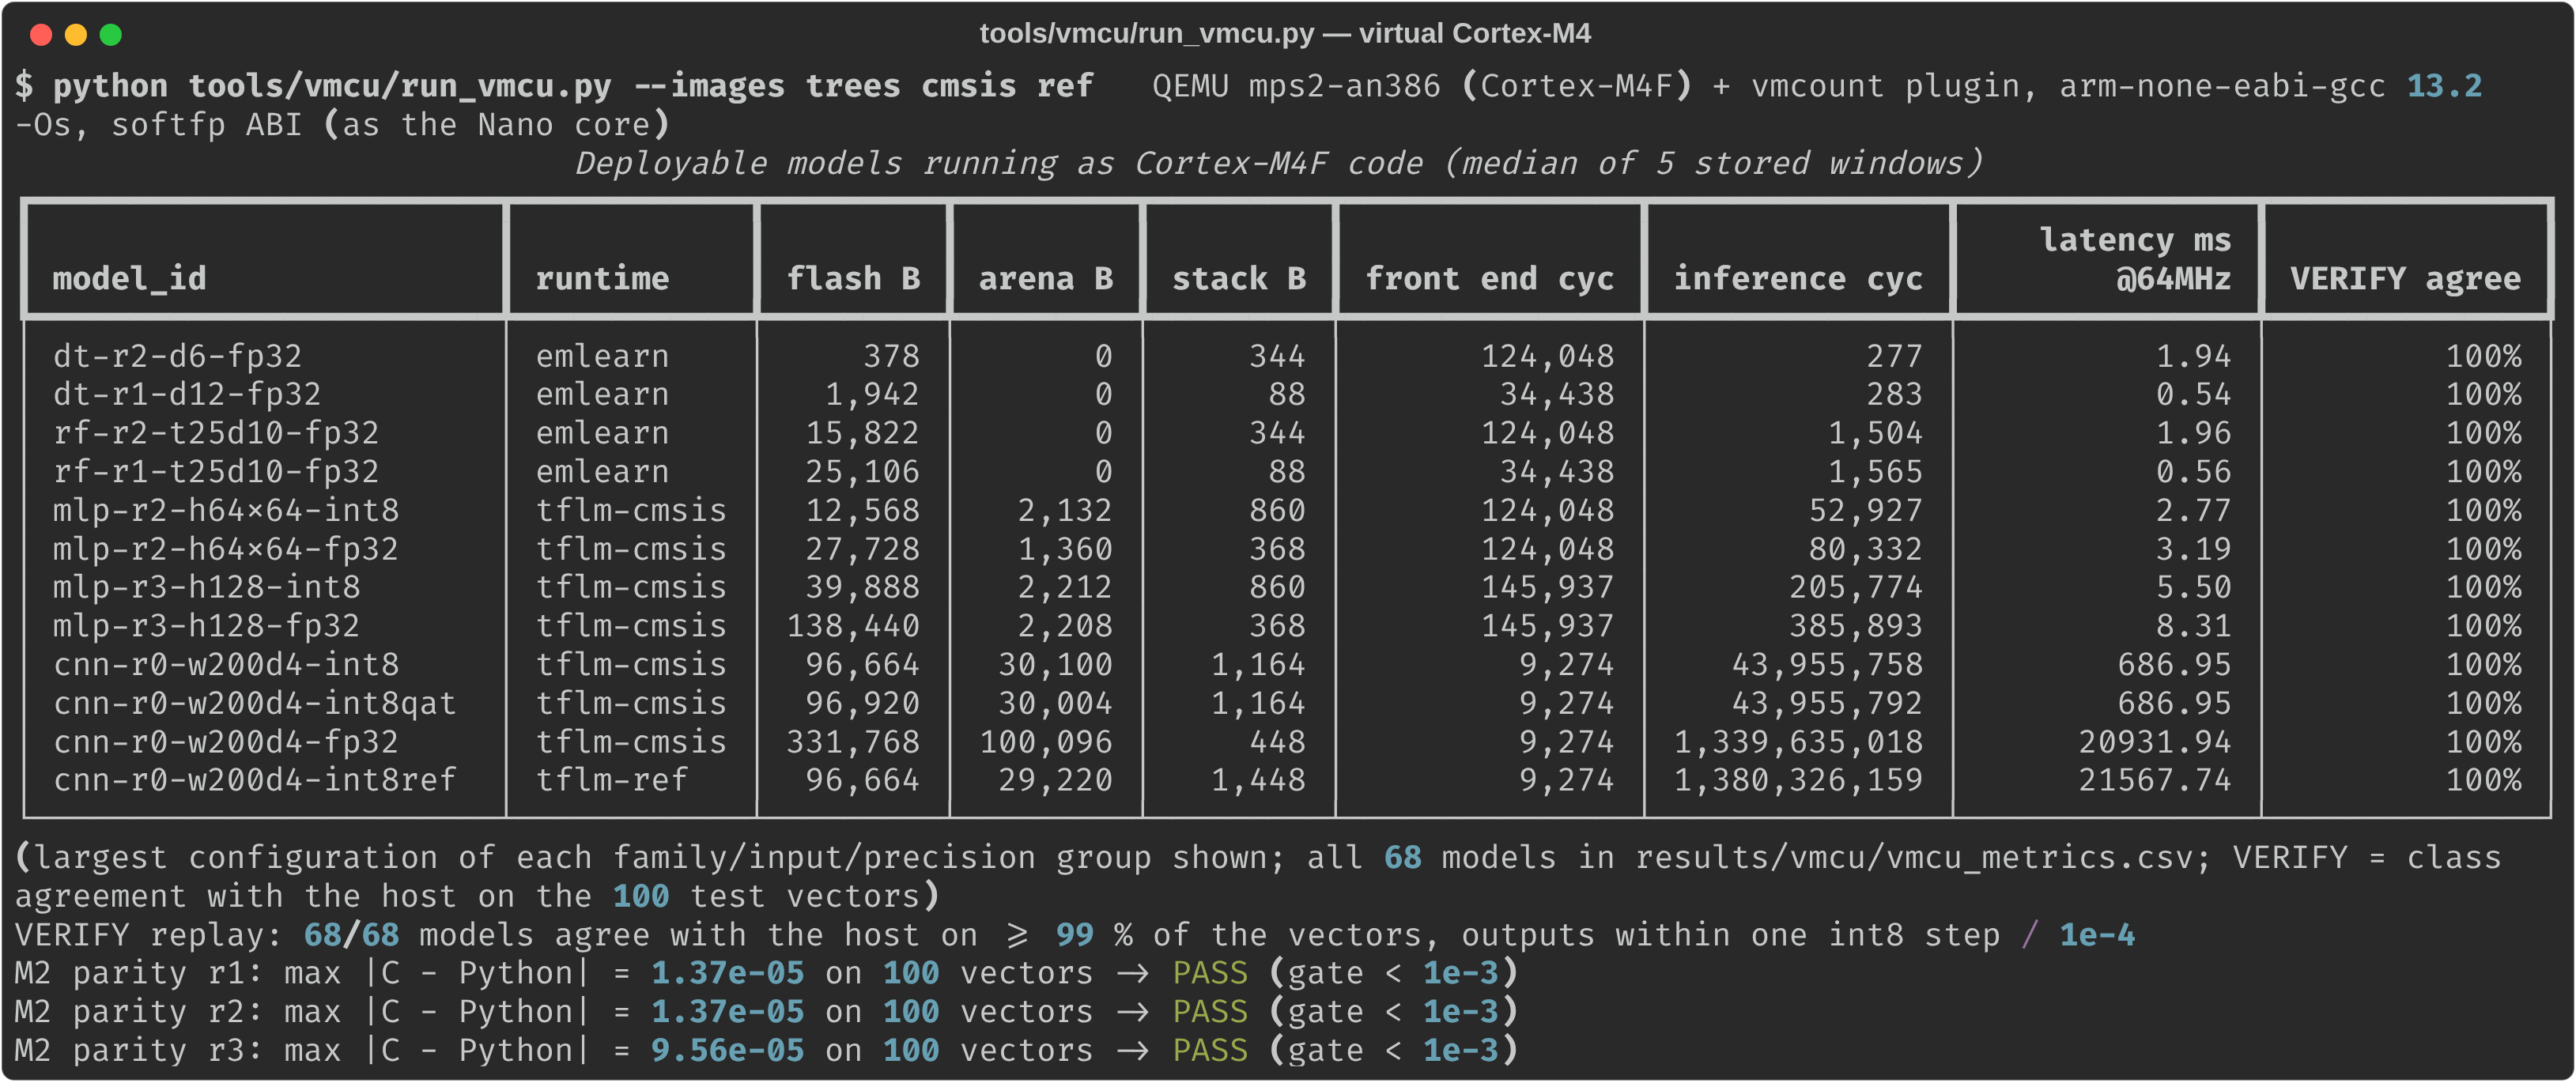
\includegraphics[width=\textwidth]{vmcu_run}\\[2pt]
{\footnotesize (a) Virtual Cortex-M4: the deployable code of every model runs as Cortex-M4F machine code in QEMU
(largest configuration of each group shown; all 68 in \texttt{results/vmcu/vmcu\_metrics.csv}).}\\[10pt]
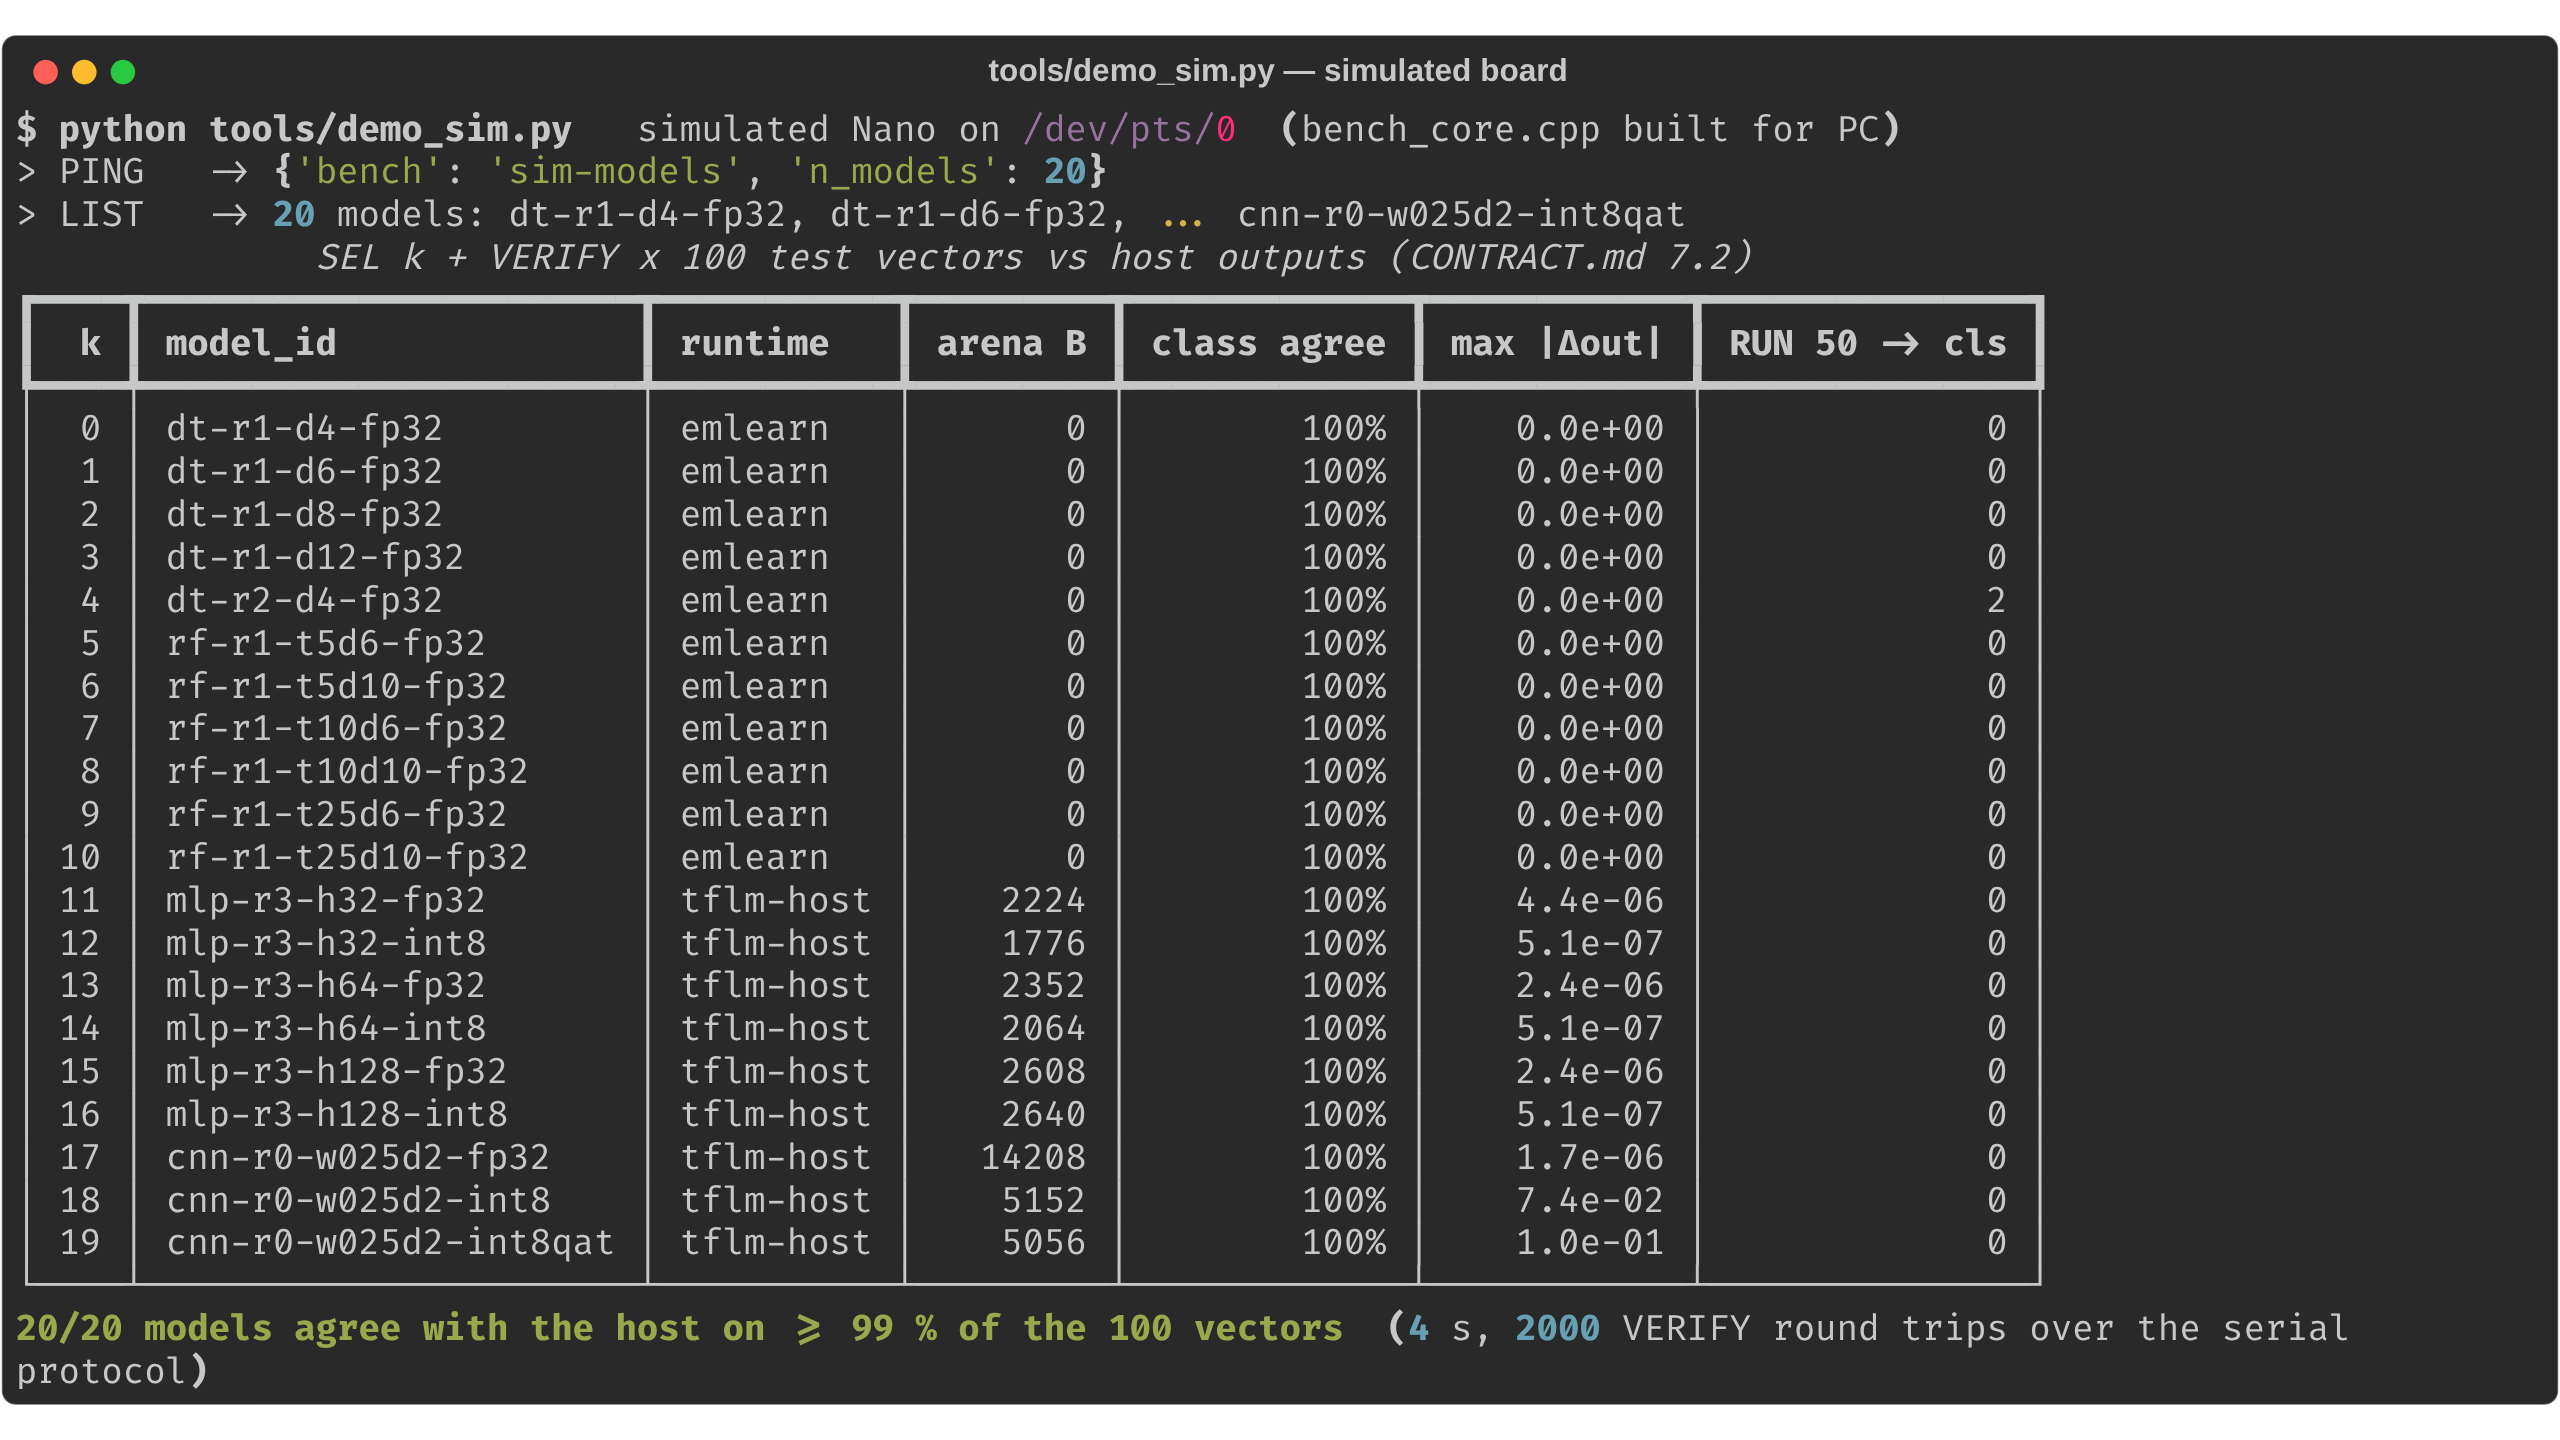
\includegraphics[width=0.82\textwidth]{demo_sim}\\[2pt]
{\footnotesize (b) Simulated board: the team's bench firmware, built for the PC with real models and the C front end,
driven over the serial protocol by \texttt{tools/dut.py} (SEL, VERIFY on the 100 test vectors, RUN).}
\caption{The two pre-hardware demonstrations. Both use the exact artefacts that will be flashed to the Nano~33~BLE.}
\label{fig:demo}
\end{figure*}

\begin{figure}[t]
\centering
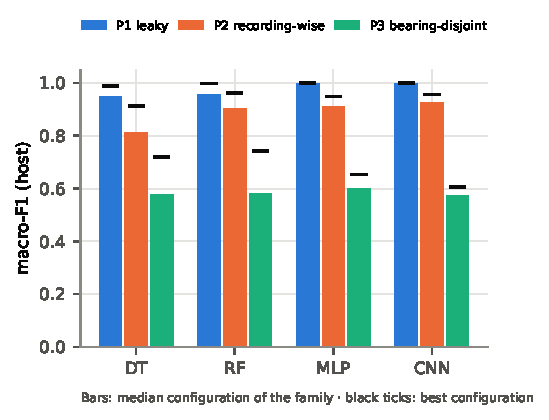
\includegraphics[width=0.86\columnwidth]{fig_protocol_drop}
\caption{Host macro-F1 per family under the three protocols (bars: median configuration; ticks: best
configuration). Mean over all folds and the seeds run so far (\NumSeedsMin{}--\NumSeedsMax{} per configuration).}
\label{fig:protocols}
\end{figure}

\subsection{Leakage changes the answer (RQ3, accuracy)}
Fig.~\ref{fig:protocols} and Table~\ref{tab:f1} summarise \NumRuns{} host runs. Under the leaky split every family
looks near-perfect (best \NumPOneBest{}). Holding out a recording (P2) costs little for the best models but separates
the families, and on unseen bearings (P3) the best model reaches only \NumPThreeBest{} macro-F1
(\NumPThreeBestModel{}), on a 4-class task. Rankings move with the protocol: Kendall's $\tau$ between the per-model
macro-F1 rankings is \NumTauModelPOnePTwo{} (P1 vs P2), \NumTauModelPOnePThree{} (P1 vs P3) and
\NumTauModelPTwoPThree{} (P2 vs P3). Bearing-disjoint scores also vary strongly across folds and seeds (standard
deviations up to \NumPThreeMLPBestStd{} in Table~\ref{tab:f1}). In this sweep, the apparent P3 winner changed
family when the MLPs went from one seed to five, so a single-seed P3 comparison is not reliable; the final
version reports every configuration over five seeds.

\begin{table}[t]
\centering
\caption{Best configuration per family: macro-F1, mean $\pm$ std over folds and seeds.}
\label{tab:f1}
\setlength{\tabcolsep}{3pt}
\begin{tabular}{lccc}
\toprule
Family & P1 leaky & P2 recording & P3 bearing \\
\midrule
DT  & \NumPOneDTBest{}$\pm$\NumPOneDTBestStd{} & \NumPTwoDTBest{}$\pm$\NumPTwoDTBestStd{} & \NumPThreeDTBest{}$\pm$\NumPThreeDTBestStd{}\\
RF  & \NumPOneRFBest{}$\pm$\NumPOneRFBestStd{} & \NumPTwoRFBest{}$\pm$\NumPTwoRFBestStd{} & \NumPThreeRFBest{}$\pm$\NumPThreeRFBestStd{}\\
MLP & \NumPOneMLPBest{}$\pm$\NumPOneMLPBestStd{} & \NumPTwoMLPBest{}$\pm$\NumPTwoMLPBestStd{} & \NumPThreeMLPBest{}$\pm$\NumPThreeMLPBestStd{}\\
CNN & \NumPOneCNNBest{}$\pm$\NumPOneCNNBestStd{} & \NumPTwoCNNBest{}$\pm$\NumPTwoCNNBestStd{} & \NumPThreeCNNBest{}$\pm$\NumPThreeCNNBestStd{}\\
\bottomrule
\end{tabular}
\end{table}

\subsection{The front end dominates feature-based models (RQ2)}
Fig.~\ref{fig:breakdown} separates the two phases on the virtual Cortex-M4. A decision tree or forest needs
\NumTreeInfMin{}--\NumTreeInfMax{} estimated cycles per window, but its R1 front end needs \NumFeROneKcyc{}\,k cycles
and its R2 front end (statistics plus a 1024-point FFT) \NumFeRTwoKcyc{}\,k: at least \NumTreeFeShareMin{} of the
end-to-end work. R0 normalisation for CNNs costs \NumFeRZeroKcyc{}\,k cycles. Counting the front end therefore moves
every feature-based model by two orders of magnitude on the energy axis, while CNNs barely move
(Fig.~\ref{fig:rq2}). This is the effect that inference-only reporting hides.

\begin{figure}[t]
\centering
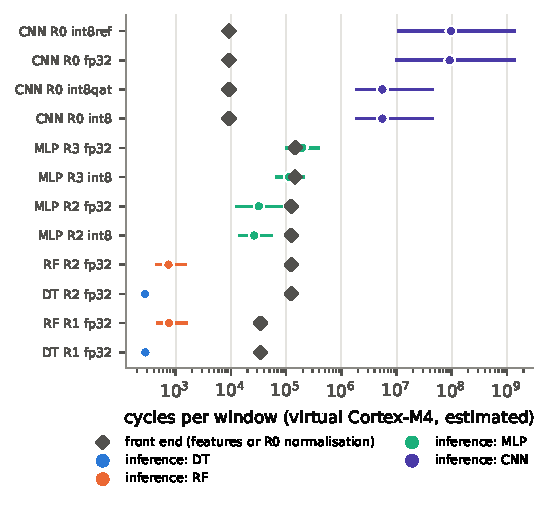
\includegraphics[width=0.86\columnwidth]{fig_energy_breakdown}
\caption{Front-end versus inference cycles per window on the virtual Cortex-M4 (median over configurations; bars
span the configurations of a group). Log scale.}
\label{fig:breakdown}
\end{figure}

\subsection{Frontiers and family dominance (RQ1, RQ3)}
Fig.~\ref{fig:pareto} shows error against estimated end-to-end energy under P2 and P3. With three objectives
(error, energy, peak RAM), the P2 frontier holds \NumFrontPTwoEtoe{} models (\NumRobustPTwoEtoe{} with bootstrap
membership probability $\geq 0.5$) and the P3 frontier \NumFrontPThreeEtoe{} (\NumRobustPThreeEtoe{}). The bootstrap
resamples test windows and draws each model's energy inside its cycle-model band (\NumBandMin{}--\NumBandMax{} wide),
so membership reflects both accuracy noise and cost-model uncertainty. Ranked by hypervolume, the families order as
\NumRankPOne{} under P1, \NumRankPTwo{} under P2 and \NumRankPThree{} under P3 (Kendall $\tau$ =
\NumTauFamPOnePTwo{}, \NumTauFamPOnePThree{} and \NumTauFamPTwoPThree{} for P1--P2, P1--P3 and P2--P3).

\begin{figure*}[t]
\centering
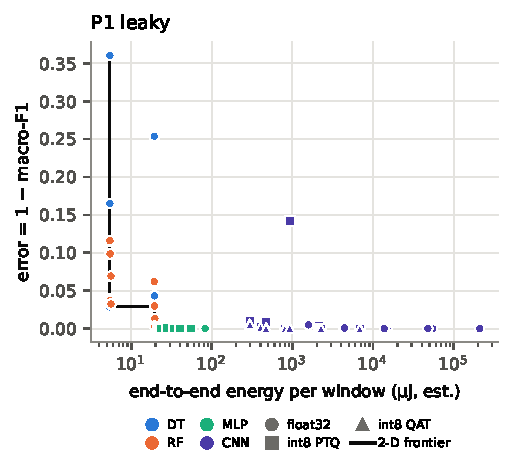
\includegraphics[width=0.32\textwidth]{fig_pareto_P1_e2e}\hfill
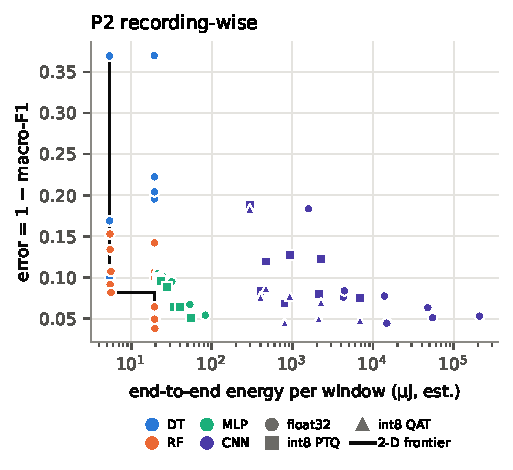
\includegraphics[width=0.32\textwidth]{fig_pareto_P2_e2e}\hfill
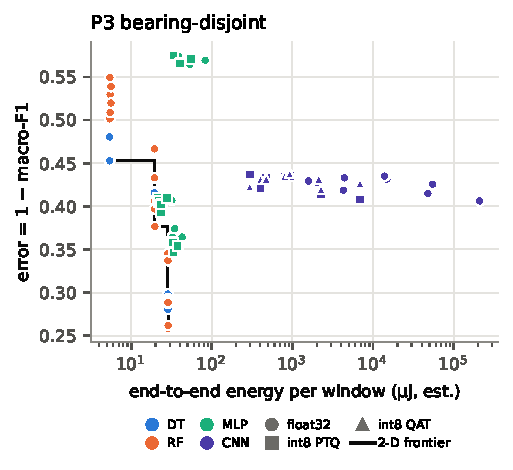
\includegraphics[width=0.32\textwidth]{fig_pareto_P3_e2e}
\caption{Error versus estimated end-to-end energy per window for every deployable configuration under P1, P2 and P3.
Colour: family; marker: precision; black staircase: two-dimensional frontier.}
\label{fig:pareto}
\end{figure*}

\begin{figure}[t]
\centering
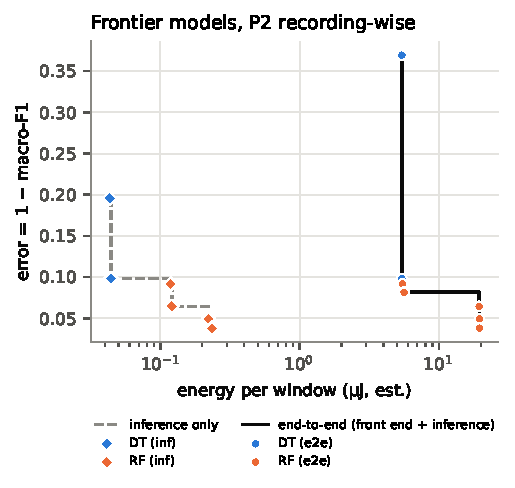
\includegraphics[width=0.86\columnwidth]{fig_rq2_frontend}
\caption{Accuracy--energy frontier members under P2 with inference-only (diamonds, dashed) and end-to-end energy
(circles, solid).}
\label{fig:rq2}
\end{figure}

\begin{table*}[t]
\centering
\caption{Pre-hardware cost on the virtual Cortex-M4 (64\,MHz, estimated) and host macro-F1 of the best P3 configuration in each family/input/precision group.}
\label{tab:costs}
\setlength{\tabcolsep}{4pt}
\begin{tabular}{lrrrrrrccc}
\toprule
Configuration & Flash (kB) & Peak RAM (kB) & Front end (kcyc) & Inference (kcyc) & Latency (ms) & Energy ($\mu$J) & P1 F1 & P2 F1 & P3 F1\\
\midrule
\texttt{dt-r1-d4-fp32} & 0.3 & 0.1 & 34.4 & 0.3 & 0.54 & 5.4 & 0.640 & 0.631 & 0.547\\
\texttt{rf-r1-t5d6-fp32} & 2.8 & 0.1 & 34.4 & 0.5 & 0.55 & 5.4 & 0.884 & 0.847 & 0.499\\
\texttt{dt-r2-d6-fp32} & 0.4 & 8.5 & 124.0 & 0.3 & 1.94 & 19.4 & 0.957 & 0.804 & 0.584\\
\texttt{rf-r2-t25d6-fp32} & 7.6 & 8.5 & 124.0 & 1.4 & 1.96 & 19.6 & 0.987 & 0.951 & 0.623\\
\texttt{mlp-r2-h64-int8} & 6.1 & 10.3 & 124.0 & 26.4 & 2.35 & 23.5 & 1.000 & 0.905 & 0.607\\
\texttt{mlp-r2-h64-fp32} & 10.4 & 9.5 & 124.0 & 32.2 & 2.44 & 24.4 & 1.000 & 0.905 & 0.608\\
\texttt{mlp-r3-h64-int8} & 20.6 & 11.5 & 145.9 & 114.0 & 4.06 & 40.6 & 1.000 & 0.935 & 0.434\\
\texttt{mlp-r3-h64-fp32} & 68.4 & 11.3 & 145.9 & 196.5 & 5.35 & 53.4 & 1.000 & 0.933 & 0.435\\
\texttt{cnn-r0-w025d2-int8qat} & 4.3 & 9.5 & 9.3 & 1887.1 & 29.63 & 295.8 & 0.988 & 0.816 & 0.600\\
\texttt{cnn-r0-w025d4-int8} & 7.9 & 10.5 & 9.3 & 2564.2 & 40.21 & 401.5 & 0.999 & 0.916 & 0.613\\
\texttt{cnn-r0-w025d4-fp32} & 10.3 & 18.2 & 9.3 & 27436.5 & 428.84 & 4281.5 & 1.000 & 0.924 & 0.614\\
\texttt{cnn-r0-w025d4-int8ref} & 7.9 & 10.5 & 9.3 & 29165.0 & 455.85 & 4551.2 & 0.999 & 0.916 & 0.613\\
\bottomrule
\end{tabular}
\end{table*}


\subsection{Kernels, precision and memory}
Table~\ref{tab:costs} lists the cost and accuracy of the best bearing-disjoint configuration of every
family/input/precision group.
On the same int8 CNNs, CMSIS-NN kernels cut estimated inference cycles by \NumCmsisMin{}--\NumCmsisMax{}$\times$
(median \NumCmsisMedian{}$\times$) relative to TFLM's reference kernels (Fig.~\ref{fig:ablation}); float CNNs, which
CMSIS-NN does not accelerate, need \NumCnnFpOverIntMin{}--\NumCnnFpOverIntMax{}$\times$ the cycles of their int8
versions. For the smallest MLPs, int8 brings no speed-up, because quantising the input and requantising each layer
cost about as much as the few hundred MACs they replace. Peak RAM (arena, feature buffers and stack) ranges from
\NumRamMinB{}\,B to \NumRamMaxKB{}\,kB, and the largest model needs \NumFlashMaxKB{}\,kB of flash.

\begin{figure}[t]
\centering
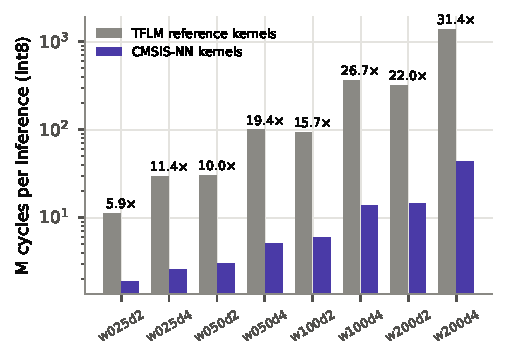
\includegraphics[width=0.86\columnwidth]{fig_cmsis_ablation}
\caption{Kernel ablation: estimated inference cycles of the int8 CNNs with TFLM reference kernels and with CMSIS-NN.}
\label{fig:ablation}
\end{figure}

\subsection{Battery life (RQ4)}
With chip-level sleep power (\SI{9.5}{\micro W}) and a CR2032 cell, the crossover rate $r^\ast$, below which sleep
dominates and the model's energy stops mattering, ranges from \NumFstarLo{}\,Hz (\NumFstarLoModel{}) to
\NumFstarHi{}\,Hz (\NumFstarHiModel{}) for the most accurate P3 model of each family (Fig.~\ref{fig:life}). At
board-level sleep power (about 3\,mW for the Nano~33~BLE), sleep dominates at every practical rate. Measuring the
board's real sleep floor is therefore part of the hardware campaign.

\begin{figure}[t]
\centering
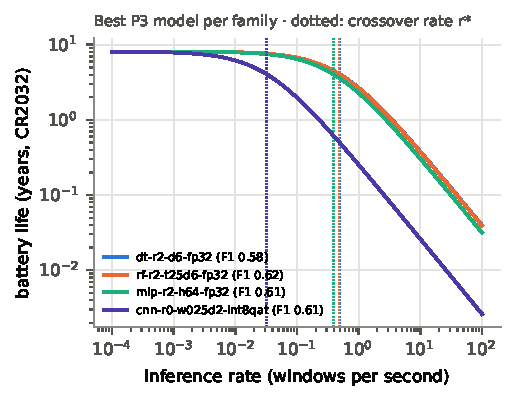
\includegraphics[width=0.86\columnwidth]{fig_lifetime}
\caption{Battery life versus inference rate for the most accurate P3 model of each family (estimated energy,
chip-level sleep). Dotted: crossover rate $r^\ast$.}
\label{fig:life}
\end{figure}

\begin{figure}[t]
\centering
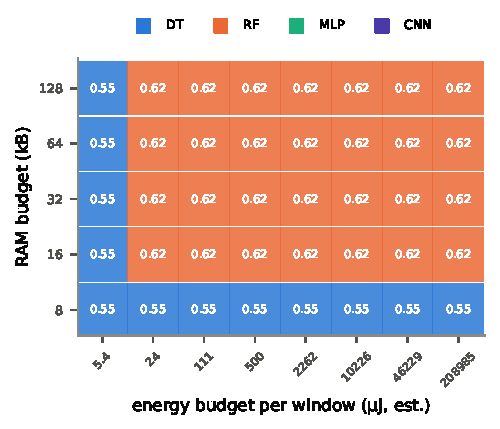
\includegraphics[width=0.8\columnwidth]{fig_rubric}
\caption{Preliminary rubric: best P3 macro-F1 (cell value) and its family (colour) under RAM and estimated-energy
budgets.}
\label{fig:rubric}
\end{figure}

\subsection{Robustness to sensor noise}
Adding white noise to the test windows separates models that clean accuracy cannot. At 0\,dB SNR under P2, the best
configuration of each family keeps a macro-F1 of \NumSnrZeroPTwoDT{} (DT), \NumSnrZeroPTwoRF{} (RF),
\NumSnrZeroPTwoMLP{} (MLP) and \NumSnrZeroPTwoCNN{} (CNN).

% =====================================================================================================================
\section{Toward a Selection Rubric}
Fig.~\ref{fig:rubric} gives the most accurate P3 model that fits each RAM and energy budget. It is the first version
of the rubric the study will deliver. The procedure: fix RAM and flash budgets; derive an energy budget from the
inference rate and the target battery life; if the rate is far below $r^\ast$, take the most accurate model that fits
RAM; otherwise take the cheapest model above the accuracy floor. Always quote bearing-disjoint (P3) accuracy, never P1.


% =====================================================================================================================
\section{Limitations and Next Steps}
This version has no board measurements. Cycles come from an instruction-exact emulator with a static Cortex-M4
timing model. Energies are proportional to cycles, so they cannot show power differences between, for example, FPU-
and integer-heavy code. The board's DWT counts (\texttt{LAT}) will calibrate the model, and
\texttt{tools/vmcu/calibrate.py} is in place for that. The INA219 rig will then replace every energy number, including
the board-level overheads (regulator, USB PHY) that the chip-level estimate omits. The virtual MCU uses current
tflite-micro and GCC~13, while the board uses Chirale's TFLM build and GCC~7, a difference the calibration will
quantify. The CNN sweep has fewer seeds than the trees so far. CWRU has a single bearing per fault class and an
artificially seeded fault, and in P3 the normal class can only be split by load. Paderborn is the planned
generalisation check.

\FloatBarrier
\section{Conclusion}
Before any hardware arrived, the full pipeline was built and gated in emulation: data, leakage-checked splits,
\NumConfigs{} deployable configurations, a virtual Cortex-M4 that runs the exact deployable code, and firmware bundles
that link for the board. The preliminary answer to the project's question is already protocol-dependent. Leaky
evaluation makes every family look interchangeable; bearing-disjoint evaluation does not. For feature-based models,
the front end, not the classifier, sets the energy cost. The hardware campaign now has to confirm these effects with
measured energy.



\bibliographystyle{IEEEtran}
\bibliography{refs}

\end{document}
